%%%%%%%%%%%%%%%%%%%%%%%%%%%%%%%%%%%%%%%%%%%%%%%%%%%%%%%%%%
%
% Master's Thesis: AI in Automotive CI/CD Pipelines
% Author: Morris Darren Babu
%
%%%%%%%%%%%%%%%%%%%%%%%%%%%%%%%%%%%%%%%%%%%%%%%%%%%%%%%%%%

\documentclass[a4paper, 12pt, headsepline, numbers=noenddot, bibliography=totoc, index=totoc, twoside, BCOR=2cm]{scrbook}

\usepackage[T2A,T1]{fontenc}
\usepackage[utf8]{inputenc}
\usepackage[slantedGreek]{mathptmx}
\usepackage[defaultsans,scale=0.99]{lato}

% usage of zapf chancery as calligraphic font instead of rsfs
% \DeclareSymbolFont{symbols}%
%   {OMS}{pzc}{m}{n}
% \DeclareSymbolFontAlphabet{\mathcal}%
%   {symbols}

\usepackage{graphicx}
\usepackage{amsmath,amsfonts,amssymb}
\usepackage{booktabs}
\usepackage{float}
% \heavyrulewidth=0.1em
\usepackage{makeidx}
\usepackage[ngerman,english]{babel}
\usepackage[autostyle]{csquotes}
\usepackage{ifthen}
\usepackage{color}

\renewcommand{\topfraction}{1.0}    % Bilder dürfen auch direkt am Seitenanfang sein
\renewcommand{\bottomfraction}{1.0} % Bilder dürfen auch direkt am Seitenende sein

\newcommand{\remark}{\tiny \normalsize}
\newcommand{\trademark}{\tiny\texttrademark \normalsize}

%%%%%%%%%%%%%%%%%%%%%%%%%%%%%%%%%%%%%%%%%%%%%%%%%%%%%%%%%%%%%%%%%%%%%%%%%%%%%%
%% NEWCOMMAND \codesigntitle
%%
%% \codesigntitle{Title}{Subtitle}{Author}{Matrikel-Nr.}{Supervisor(s)}
%%%%%%%%%%%%%%%%%%%%%%%%%%%%%%%%%%%%%%%%%%%%%%%%%%%%%%%%%%%%%%%%%%%%%%%%%%%%%%
\newcommand{\codesigntitle}[5]{%
  \begin{titlepage}
    \titlehead{%
      \hspace*{-18mm}%
      \parbox[t]{14.4cm}{%
        \parbox{76mm}{%
          \vspace*{-28mm}%
          
\includegraphics[width=35mm]{bilder/codesign}%
        }%
        \hfill
        \parbox{20mm}{%
          \vspace*{-20mm}%
          
\includegraphics[width=58mm]{bilder/FAU_TechFak_H_PMS_blue_crop}%
        }%
      }%
    }%
    \title{%
      {\parbox{0mm}{}\\[1cm]\huge\sffamily\bfseries#1}\\[4mm]
      \Huge#2%
    }%
    \ifthenelse{\boolean{englishDocument}}{%
      \author{%
        \Large by\\[4mm]
        \Large\bfseries#3\\[2mm]
        \large Matrikel-Nr.: #4\\[7mm]
        \Large Supervision:\\#5\\[16mm]
      }%
      \date{\dateenglish{\today}}%
    }{%
      \author{%
        \Large von\\[4mm]
        \Large\bfseries#3\\[2mm]
        \large Matrikel-Nr.: #4\\[7mm]
        \Large Betreuung:\\#5\\[16mm]
      }%
      \date{\datengerman{\today}}%
    }%
    \thispagestyle{empty}%
    \ifthenelse{\boolean{englishDocument}}{%
      \lowertitleback{This document was produced with the typesetting system \LaTeX2e.}%
    }{%
      \lowertitleback{Dieses Dokument wurde mit dem Textsatzsystem \LaTeX2e erstellt.}%
    }%
  \end{titlepage}%
  \maketitle
}

\newboolean{printVersion}
\setboolean{printVersion}{true}      % default setting
\newboolean{englishDocument}
\setboolean{englishDocument}{false}  % default setting

\makeindex


% --- DOCUMENT CONFIGURATION ---
\setboolean{englishDocument}{true}
\newcommand{\studname}{Morris Darren Babu}

% --- PACKAGES ---
\usepackage{graphicx}
\usepackage{booktabs}
\usepackage{longtable}
\usepackage{listings}
\usepackage{xcolor}
\usepackage{enumitem}
\usepackage{tikz}     
% Required for V-Model diagram and architecture diagrams
\usetikzlibrary{positioning, arrows.meta, shapes.geometric, fit, backgrounds, calc}
\usepackage[hyphens]{url}

% --- HYPERLINK SETUP ---
\usepackage[colorlinks=true, 
    linkcolor=blue, 
    citecolor=blue, 
    urlcolor=blue,
    pdftitle={AI Usage in CI/CD/CT Pipelines},
    pdfauthor={Morris Darren Babu}
]{hyperref}

% --- BIBLIOGRAPHY SETUP ---
\usepackage[backend=biber, 
    style=numeric, 
    maxnames=80, 
    minnames=4, 
    giveninits=false, 
    defernumbers=true, 
    maxcitenames=2, 
    mincitenames=1, 
    bibencoding=utf8
]{biblatex}
\addbibresource{literature.bib} 

% --- CODE STYLING ---
\definecolor{codegray}{rgb}{0.5,0.5,0.5}
\definecolor{codeblue}{rgb}{0,0,0.6}
\definecolor{codegreen}{rgb}{0,0.5,0}

\lstdefinestyle{codestyle}{
    backgroundcolor=\color{white},   
    commentstyle=\color{codegreen},
    keywordstyle=\color{blue},
    stringstyle=\color{codeblue},
    basicstyle=\ttfamily\footnotesize,
    breakatwhitespace=false,         
    breaklines=true,                 
    captionpos=b,                    
    keepspaces=true,                 
    numbers=left,                    
    numbersep=5pt,                  
    showspaces=false,                
    showstringspaces=false,
    showtabs=false,                  
    tabsize=2,
    frame=single,
    framerule=0.1pt,
    framesep=3pt,
    rulecolor=\color{black}
}
\lstset{style=codestyle}

\begin{document}

\ifthenelse{\boolean{englishDocument}}{\selectlanguage{english}}{\selectlanguage{ngerman}}

% =========================================
% FRONT MATTER
% =========================================
\frontmatter

\codesigntitle{Master's Thesis}
{AI Usage in CI/CD/CT Pipelines for Compute Platforms in Automotive}
{\studname}
{08150815} % <<<--- REMINDER: CHECK MATRIKEL-NR
{University Supervisor: \\
Prof. Dr.-Ing. Jürgen Teich\\
Dr.-Ing. Stefan Wildermann\\[4mm]
Industrial Supervisor (CARIAD SE): \\
Dr.-Ing. Bernd Schaller\\
Dr. Andreas Weichslgartner}

% Aufgabenstellung page
% If your program requires the official Aufgabenstellung, replace the text below
% with the official version provided by your examination office.
\addchap*{Aufgabenstellung zur Masterarbeit}

\textbf{Thema:} AI Usage in CI/CD/CT Pipelines for Compute Platforms in Automotive

\vspace{0.5cm}

\textbf{Aufgabenstellung:}

Modern automotive software systems exceed 100 million lines of code per vehicle, creating significant challenges for security testing at scale. Fuzz testing is an effective technique for discovering software vulnerabilities, but writing fuzz drivers requires deep API knowledge and considerable manual effort. This thesis investigates whether Large Language Models (LLMs) can automate fuzz driver generation for C/C++ automotive libraries and whether the resulting approach is viable for enterprise CI/CD pipelines.

The following tasks shall be addressed:

\begin{enumerate}
    \item \textbf{Literature Review:} Survey the state of the art in LLM-based code generation, fuzz testing techniques, and CI/CD pipeline security integration. Identify research gaps for automotive applications.

    \item \textbf{Framework Design:} Design a technical framework for automated LLM-based fuzz driver generation, comprising automated API context extraction, prompt construction, and coverage-based evaluation.

    \item \textbf{Empirical Evaluation:} Systematically evaluate multiple open-source LLMs (varying in size, architecture, and specialization) on their ability to generate compilable, executable, and coverage-achieving fuzz drivers for C++ libraries.

    \item \textbf{Model Optimization:} Investigate whether domain-specific fine-tuning (LoRA) of smaller models can match or exceed larger general-purpose models in fuzz driver quality and efficiency.

    \item \textbf{Enterprise Integration:} Deploy and validate the approach within a real automotive enterprise CI/CD environment (CARIAD SE), addressing network isolation, security compliance, and cost constraints.

    \item \textbf{Analysis and Discussion:} Analyze the results with respect to effectiveness, optimization potential, and enterprise feasibility. Discuss limitations, implications for practice, and future research directions.
\end{enumerate}

\vspace{0.5cm}
\noindent\textbf{Bearbeitungszeitraum:} Mai 2025 -- September 2025
 
\chapter*{Abstract}

Modern automotive software exceeds 100 million lines of code per vehicle, making thorough security testing essential under ISO~26262 and UNECE~WP.29 regulations. Fuzz testing is effective at discovering software vulnerabilities, but writing fuzz drivers requires deep API knowledge, a capability that many development teams lack.

This thesis investigates whether Large Language Models (LLMs) can automate fuzz driver generation for C/C++ automotive libraries and whether the approach is viable for enterprise CI/CD pipelines.

We evaluated 14 open-source LLMs ranging from 1.5 to 46.7 billion parameters on the \texttt{yaml-cpp} library and additional C++ targets. The results revealed a counterintuitive pattern: larger models did not perform better. General-purpose models such as Yi (34B) failed to produce functional fuzz drivers, and Mixtral (46.7B) could not be fully evaluated due to hardware constraints. In contrast, Gemma~3 (27B) achieved approximately 45\% line coverage, and the code-specialized Qwen~2.5-Coder (32B) reached approximately 43\%. Notably, several explicitly code-specialized models such as CodeLlama (34B) also failed, demonstrating that neither model size nor a code-specialization label alone predicts success for this task.

To address resource constraints, we fine-tuned a compact 1.5B-parameter model using Low-Rank Adaptation (LoRA) on fuzz drivers extracted from Google's OSS-Fuzz project. Fine-tuning reduced generation time by 33\% and token usage by 55\% while maintaining driver quality, making deployment in resource-constrained environments practical.

Enterprise integration at CARIAD~SE revealed that infrastructure challenges can rival the technical ones. Corporate firewalls blocked external API calls from isolated CI/CD runners, requiring an architectural solution based on Azure Private Link and self-hosted runners. This experience demonstrates that production deployment depends as much on infrastructure planning as on model quality.

An economic analysis shows that full enterprise deployment costs approximately \euro{}1,500 annually, a modest investment compared to the cost of manual security engineering. Overall, LLM-based fuzz driver generation is both technically viable and cost-effective for automotive security, provided the model is chosen carefully and infrastructure is adapted to enterprise constraints.

\vspace{1cm}
\noindent \textbf{Keywords:} Large Language Models, Fuzz Testing, Automotive Security, CI/CD Integration, LoRA Fine-Tuning, ISO~26262, Code Coverage.

% --- TABLE OF CONTENTS ---
\tableofcontents

% --- LISTS ---
% This command automatically searches all chapters for \begin{figure} and lists them here
\cleardoublepage
\phantomsection
\addcontentsline{toc}{chapter}{List of Figures}
\listoffigures

\cleardoublepage
\phantomsection
\addcontentsline{toc}{chapter}{List of Tables}
\listoftables

\cleardoublepage
\phantomsection
\addcontentsline{toc}{chapter}{List of Abbreviations}
\chapter*{List of Abbreviations}
\begin{itemize}
    \item[ABS] Anti-lock Braking System
    \item[ADAS] Advanced Driver-Assistance Systems
    \item[AFL] American Fuzzy Lop
    \item[AI] Artificial Intelligence
    \item[API] Application Programming Interface
    \item[ASan] AddressSanitizer
    \item[AST] Abstract Syntax Tree
    \item[AUTOSAR] AUTomotive Open System ARchitecture
    \item[BRS] Business Requirements Specification
    \item[CD] Continuous Delivery / Continuous Deployment
    \item[CI] Continuous Integration
    \item[CT] Continuous Testing
    \item[DNS] Domain Name System
    \item[ECU] Electronic Control Unit
    \item[GPU] Graphics Processing Unit
    \item[HLD] High-Level Design
    \item[JSON] JavaScript Object Notation
    \item[LLD] Low-Level Design
    \item[LLM] Large Language Model
    \item[LLVM] Low Level Virtual Machine
    \item[LoRA] Low-Rank Adaptation
    \item[MTTV] Mean Time To Vulnerability
    \item[SAE] Society of Automotive Engineers
    \item[SRS] System Requirements Specification
    \item[UBSan] UndefinedBehaviorSanitizer
    \item[UNECE] United Nations Economic Commission for Europe
    \item[XML] Extensible Markup Language
    \item[YAML] YAML Ain't Markup Language
\end{itemize}

% =========================================
% MAIN MATTER
% =========================================
\mainmatter

% Using your specific filenames
% File: chapters/chapter1_introduction.tex

\chapter{Introduction}
\label{chap:introduction}

\section{Background and Motivation}
\label{sec:background_motivation}

Automotive software has changed fundamentally in the last 15 years. When I first read about vehicle cybersecurity, I was surprised to learn that a modern car runs over 100 million lines of code. Not thousands. Not millions. Over 100 million. Distributed across more than 100 Electronic Control Units (ECUs). This number, which appears in industry reports \cite{Charette2009, Broy2006}, illustrates a complete shift in how we think about vehicles.

This shift came from somewhere. Vehicles used to be mechanical systems. An engine controller managed fuel injection. An ABS system prevented wheel lockup. These systems mostly operated independently. A skilled engineer could understand the complete electronic architecture within weeks. That is gone now.

Today, vehicles are software platforms that happen to have wheels. Tesla demonstrated this most clearly. When Tesla updates a vehicle over the air, customers receive new features, better performance, and improved safety. All without visiting a service center. Traditional automakers watched this happen and realized something fundamental had changed. Software now determines competitive advantage. It determines how fast a car accelerates. It determines what features customers receive. Mechanical engineering no longer drives differentiation.

This transformation created a problem. Software is complex. A single vehicle contains code spanning multiple programming paradigms, different safety criticality levels, and various execution environments. Code that is safety-critical on AUTOSAR platforms follows entirely different development rules than infotainment applications running on Linux. Real-time control systems operating at microsecond intervals coexist with cloud-connected services. This diversity makes testing exponentially harder.

Consider a Level 2 automated driving system. Perception algorithms process camera, radar, and lidar data. Planning modules compute safe trajectories. Control systems translate trajectories into steering and throttle commands. Each layer requires different technical expertise: computer vision, machine learning, control theory, real-time systems. Integration alone consumes enormous effort. When you add legacy code to this, code written years ago with minimal documentation, understanding what the software actually does becomes detective work.

\subsection{Security Challenges in Modern Systems}
\label{sec:security_challenges}

This complexity creates security risks that are genuinely dangerous. When a web server gets compromised, the consequences are serious. Data theft, service disruption, financial loss. When a vehicle control system is compromised, it can result in severe physical harm or fatal injuries. This is not theoretical. In 2015, researchers demonstrated remote exploitation of a Jeep Cherokee. They showed scenarios where attackers could disable brakes or seize steering at highway speeds \cite{MillerValasek2015}. Chrysler recalled 1.4 million vehicles. The infotainment system, connected via cellular networks, had provided a pathway to safety-critical networks.

Regulators noticed a critical security gap in vehicle software. UNECE Regulation 155 now requires cybersecurity management systems for all new vehicle types \cite{UNECER155}. ISO/SAE 21434 sets cybersecurity engineering requirements across the entire vehicle lifecycle \cite{ISO21434}. These are not suggestions. Vehicles that do not comply cannot be sold in regulated markets. Manufacturers must demonstrate that security was designed into systems from the beginning, not bolted on afterward.

This regulatory pressure collides with a fundamental tension in automotive security testing. Safety-critical systems undergo exhaustive verification against precisely defined requirements, like ISO 26262 \cite{ISO26262}. Every possible failure mode is analyzed. Fixes are tested. This works for safety, where hazards are known and physics are deterministic.

Security is different. The adversary is intelligent, creative, and unconstrained by specifications. Attackers do not limit themselves to documented interfaces. They probe for implementation weaknesses, logic errors, overlooked edge cases. Testing for security means exploring the unexpected, not verifying the expected. This requires fundamentally different approaches.

\subsection{Fuzzing}
\label{sec:fuzzing}

\begin{figure}[htbp]
    \centering
    \resizebox{\textwidth}{!}{
    \begin{tikzpicture}[
        databox/.style={draw, rectangle, minimum width=3.8cm, minimum height=1cm, align=center, fill=blue!8, thick, font=\small},
        procbox/.style={draw, rounded corners=8pt, rectangle, minimum width=3.8cm, minimum height=1cm, align=center, fill=orange!12, thick, font=\small},
        arrow/.style={->, >=stealth, thick},
        every node/.style={inner sep=6pt}
    ]
    % --- ROW 1: Developer inputs ---
    \node[databox] (srccode) at (0,0) {Source Code};
    \node[databox] (domknow) at (5.5,0) {Domain Knowledge};

    % --- ROW 2: Manual driver writing (bottleneck) ---
    \node[procbox, fill=red!15] (driverwrite) at (2.75,-2) {\textbf{Manual Fuzz Driver}\\\textbf{Creation} {\footnotesize(bottleneck)}};

    % --- ROW 3: Fuzz Driver ---
    \node[databox] (fuzzdriver) at (2.75,-4) {Fuzz Driver};
    \node[databox] (seedinputs) at (8,-4) {Seed Inputs};

    % --- ROW 4: Fuzzing Engine ---
    \node[procbox] (fuzzengine) at (5,-6) {Fuzzing Engine\\{\footnotesize(libFuzzer / AFL++)}};

    % --- ROW 5: Outputs ---
    \node[databox] (crashdata) at (1.5,-8.5) {Crash Data};
    \node[databox] (covdata) at (8.5,-8.5) {Coverage Data};

    % --- ROW 6: Processing ---
    \node[procbox] (vuln) at (1.5,-10.5) {Vulnerability Report\\Generation};
    \node[procbox] (mutate) at (8.5,-10.5) {Input Mutation};

    % --- ROW 7: Final outputs ---
    \node[databox] (vulnreport) at (1.5,-12.5) {Vulnerability Report};
    \node[databox] (mutinputs) at (8.5,-12.5) {Mutated Inputs};

    % --- ARROWS ---
    \draw[arrow] (srccode) -- (driverwrite);
    \draw[arrow] (domknow) -- (driverwrite);
    \draw[arrow] (driverwrite) -- (fuzzdriver);
    \draw[arrow] (fuzzdriver) -- (fuzzengine);
    \draw[arrow] (seedinputs) -- (fuzzengine);
    \draw[arrow] (fuzzengine) -- (crashdata);
    \draw[arrow] (fuzzengine) -- (covdata);
    \draw[arrow] (crashdata) -- (vuln);
    \draw[arrow] (covdata) -- (mutate);
    \draw[arrow] (vuln) -- (vulnreport);
    \draw[arrow] (mutate) -- (mutinputs);

    % --- Feedback loop ---
    \draw[arrow] (mutinputs.east) -- ++(1.2,0) |- (fuzzengine.east);

    \end{tikzpicture}
    }
    \caption{The Fuzzing Process. Data artifacts are shown in rectangular boxes; processing steps are shown in rounded boxes. The manual creation of fuzz drivers (highlighted in red) is the bottleneck this thesis aims to automate.}
    \label{fig:fuzzing_concept}
\end{figure}

The fuzzing architecture begins with the human element. The developer writes the initial source code and possesses the critical domain knowledge required to understand the intended software logic. Because an automated system cannot inherently know what specific areas to target, the developer must manually define the testing scope and create the fuzz driver, a small program that translates raw fuzzer inputs into meaningful API calls. This manual creation step requires significant effort and specialized expertise, representing the primary bottleneck that this research aims to automate.

Once the fuzz driver and seed inputs are supplied, the automated fuzzing engine takes control. As illustrated in Figure~\ref{fig:fuzzing_concept}, the engine continuously executes the fuzz driver against the target software, feeding it generated inputs while actively monitoring for unexpected behavior. If a crash is detected, the engine extracts the crash data, and a vulnerability report is generated. Conversely, if the execution completes without error, the engine collects coverage data to understand which code paths were reached. An input mutation step then creates slightly altered variations of the previous inputs. These mutated inputs are fed back into the execution loop, driving a continuous cycle of automated vulnerability discovery.


\subsection{CI/CD Pipeline Context}
\label{sec:cicd_context}

Modern software development has embraced a philosophy: integrate code frequently, test automatically, deploy rapidly. The reasoning is sound. Small, incremental changes are easier to understand and debug than large infrequent releases. Automated testing catches regressions before they spread. Fast feedback loops let developers address problems while context is fresh \cite{Humble2010, Fowler2006}.

The automotive industry has adopted these principles, adapting them to domain-specific constraints. You do not casually push untested code to vehicles traveling at highway speeds. Automotive continuous integration pipelines typically feed into formal release processes with human review and additional validation before software reaches production vehicles.

But the core principles hold: automate what you can, test early and often, maintain a continuously releasable codebase \cite{CiCdFuzzing2022}.

\begin{figure}[htbp]
    \centering
    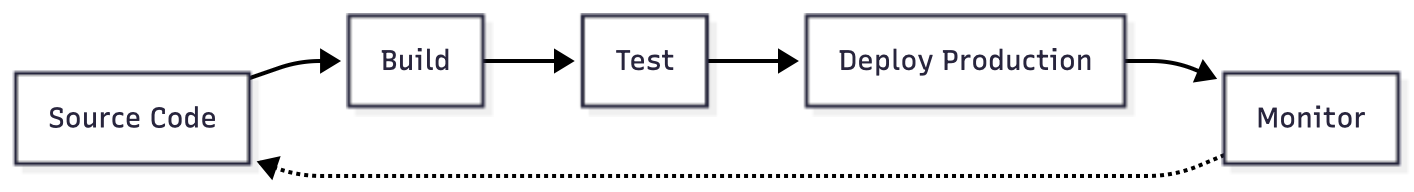
\includegraphics[width=\textwidth]{bilder/cicd.png}
    \caption{The Automotive CI/CD Pipeline. The diagram illustrates the stages from code commit through deployment, highlighting where security validation typically occurs.}
    \label{fig:cicd_pipeline}
\end{figure}

This creates a tension. A well-optimized pipeline might complete build and basic testing in 15 to 30 minutes. Developers expect rapid feedback. But security testing, especially fuzzing, often requires extended execution. A fuzzing campaign might run for hours or days to discover subtle vulnerabilities \cite{OSSFuzzBugs2021}. This timescale is incompatible with developer expectations for fast feedback.

Enterprise environments add additional complexity. Large organizations balance computational demands against security requirements. Build runners may execute in public cloud for scalability while sensitive operations stay in private networks isolated from external connections \cite{AzureDevOps}. Network policies restrict communication between zones. A simple task like calling an LLM API from a build runner encounters firewalls, proxy servers, and access control systems.


\section{Problem Statement}
\label{sec:problem_statement}

The core problem is straightforward: code production vastly outpaces security analysis capacity.

In the broader automotive software industry, massive development teams deploy continuous code modifications. For example, at CARIAD, hundreds of developers produce thousands of changes daily. Even well-staffed security teams cannot review each change for vulnerabilities. Automated tools like SonarQube, Coverity, and Checkmarx provide assistance, but static analysis frequently generates false positives that require manual human triage, and dynamic analysis requires test harnesses that must be created manually.

Fuzzing attempts to bypass this manual review bottleneck, though it introduces a different limitation. Google's OSS Fuzz project has found over 10,000 vulnerabilities in open source software through continuous fuzzing \cite{OSSFuzzBugs2021, LibFuzzer2015}. The effectiveness of this approach is extensively documented. The constraint is fuzz driver creation.

A fuzz driver is a small program that feeds generated inputs to target functionality. Writing effective drivers requires understanding API contracts, identifying interesting code paths, and constructing inputs that explore edge cases. This is specialized work. While the automotive software industry employs specialists capable of writing these drivers, the available workforce cannot scale to match the massive volume of daily code production required by major manufacturers.

The mismatch creates a security gap. Code ships with inadequate fuzzing coverage. Vulnerabilities that could have been discovered through systematic fuzzing remain hidden until attackers find them or security incidents force discovery.

Large Language Models offer a potential solution. These models, trained on vast amounts of source code, can generate syntactically correct code following common patterns \cite{Touvron2023, Bai2023}. Recent research shows LLM capabilities in various software engineering tasks: code completion, bug detection, test generation, documentation \cite{TitanFuzz2022, Fuzz4All2023}.

The question we asked was simple: can LLMs generate fuzz drivers? Specifically, can they generate drivers that compile, execute without crashing, and achieve meaningful code coverage?

This question mattered to us at CARIAD because if the answer was yes, it could change how we approach security testing at scale.

\section{Research Questions and Objectives}
\label{sec:rq_objectives}

We had three main research questions driving this work.

\subsection{Primary Research Questions}
\label{sec:primary_rq}

\textbf{RQ1 (Effectiveness): Can Large Language Models generate fuzz drivers for C++ code that compile successfully, execute without errors, and achieve meaningful code coverage?}

This is the fundamental question. A driver that fails to compile is useless. One that compiles but crashes immediately provides no security value. A driver that runs but only exercises trivial code paths does not justify its existence. Meaningful coverage means reaching error handling paths, boundary conditions, and complex interaction sequences \cite{LLMDriverGenEffectiveness2023}.

\textbf{RQ2 (Optimization): Does model size determine fuzz driver quality, or can smaller models with domain-specific training match or exceed larger general purpose models?}

Everyone in machine learning hears that bigger models are better. Models with more parameters consistently outperform smaller ones on standard benchmarks \cite{Jiang2023}. The largest models show impressive capabilities across diverse tasks. They are also expensive, require substantial compute, and often have rate limits. But domain-specific tuning offers an alternative path \cite{Hu2021}. Instead of relying on the general knowledge of massive models, we adapt smaller models to specific tasks.

We wanted to know: which approach wins for fuzz driver generation?

\textbf{RQ3 (Feasibility): Can LLM-assisted fuzz driver generation be integrated into secure enterprise CI/CD pipelines that are isolated from external networks while meeting performance, cost, and security requirements?}

Academic research often evaluates techniques in isolation, abstracting away deployment concerns. Production matters. Can the solution run within CI/CD time constraints? Does the cost fit budget limits? Can it operate under network security policies that restrict external communication? Is operational complexity acceptable?

These questions drove our entire investigation. We were not just asking whether LLMs could generate code. We were asking whether this approach could work in a real company, dealing with real constraints.

\section{Thesis Organization}
\label{sec:thesis_organization}

The rest of this thesis is structured as follows.

\textbf{Chapter 2: Literature Review} surveys relevant research. It examines traditional AI approaches in software testing, traces the evolution of Large Language Models and their application to code generation, reviews fuzzing techniques from foundational methods through AI-enhanced approaches, and examines prior work on security integration in CI/CD pipelines.

\textbf{Chapter 3: Methodology and Framework} presents our approach. It introduces the conceptual framework for AI-driven fuzzing using white-box techniques, describes our technical architecture design, and outlines the three research phases: local LLM evaluation, model optimization with LoRA, and enterprise CI/CD integration. We specify evaluation methodology and metrics.

\textbf{Chapter 4: Implementation} covers the concrete realization. It addresses toolchain selection, describes experimental setup for each phase, documents architectural challenges encountered during enterprise integration, and explains how we solved them.

\textbf{Chapter 5: Experimental Results} presents empirical findings: results of fuzz driver generation across evaluated models, performance variations across target repositories, model optimization outcomes, and economic analysis.

\textbf{Chapter 6: Discussion and Conclusion} interprets results against our research questions. It examines what the data reveals about LLM capabilities, addresses unexpected findings, acknowledges limitations, explores implications for automotive industry practice, synthesizes contributions, and identifies future research directions.
% File: chapters/chapter2_literature.tex

\chapter{Literature Review}
\label{chap:literature_review}

\section{Traditional AI Approaches in Software Testing}
\label{sec:lit_traditional_ai}

Automated software testing has been a research area for decades, and AI techniques have played various roles in its evolution. Understanding the historical context helps explain why LLM-based approaches represent a different class of methods.

\textbf{Genetic algorithms} were among the earliest AI applications to testing. The basic idea was straightforward: treat test case generation as an optimization problem. Maintain a population of test cases, apply selection and mutation operations across generations, and let evolution guide toward more effective tests. Wang et al. documented how evolutionary testing dominated research from the late 1990s through the early 2010s \cite{MLFuzzReview2020}.

This approach showed initial promise. Coverage could be formulated as a fitness function. Generate test cases that maximize coverage. Multi-objective optimization helped balance competing goals. Over time, limitations became apparent. Fitness function design proved challenging. Maximizing code coverage did not necessarily correlate with bug detection. Most fundamentally, genetic algorithms lacked semantic understanding. They could shuffle bytes and hope for improvements, but they could not understand what made certain inputs meaningful for a particular API.

\textbf{Symbolic execution} offered a different approach based on constraint solving rather than random search. The technique treats program inputs as symbolic values and accumulates path constraints during execution. Solving these constraints yields concrete inputs guaranteed to exercise specific program paths. Microsoft's SAGE, deployed internally for security testing, demonstrated practical viability by finding vulnerabilities that conventional testing had missed \cite{SAGE2008}.

Symbolic execution offers theoretical rigor. But it faces serious scalability problems. The number of paths through a program grows exponentially with the number of branch points. This is the path explosion problem. Yavuz's recent work on DESTINA addresses this through targeted execution strategies, but complete path coverage remains infeasible for realistic programs \cite{DESTINA2024}.

\textbf{Machine learning entered testing} in supporting roles around 2015. A Sandia National Laboratories report surveyed early applications: defect prediction, test case prioritization, coverage estimation \cite{MLFuzzReviewSandia2019}. These applications used ML models to inform human decisions rather than generate tests directly. They were practical and useful but did not fundamentally change how tests were created.

Neural networks enabled more ambitious applications. Pei et al. introduced DeepXplore for testing deep learning systems, defining neuron coverage as a testing adequacy criterion \cite{DeepXplore2017}. Odena et al. extended coverage-guided fuzzing to neural networks with TensorFuzz \cite{TensorFuzz2019}. These works showed that neural networks could participate actively in testing rather than merely supporting it.

This context shows why LLM-based approaches represent a different class of methods. Previous AI techniques either optimized based on metrics (genetic algorithms, coverage-guided fuzzing) or reasoned about program structure (symbolic execution). LLMs do something different: they learn patterns from vast code repositories and can generate syntactically correct code following those patterns.

\section{Large Language Models: Evolution and Code Generation}
\label{sec:lit_llm_evolution}

The Transformer architecture, introduced in 2017, enabled training on vastly larger datasets than previous approaches permitted. Scaling revealed that models trained on next-token prediction could perform diverse tasks.

GPT-3 (2020) demonstrated this principle. With 175 billion parameters, it could write coherent text and syntactically valid code. The specific finding that mattered for software engineering: the model had learned patterns from code in its training data and could apply them to generate new code.

Code-specific models followed. Codex, which powers GitHub Copilot, achieved 28.8\% success on the HumanEval benchmark initially and 70.2\% with multiple sampling attempts \cite{Chen2021}. GPT-4 further improved code generation with better contextual understanding and reduced subtle errors. Context windows expanded from 2K to 128K tokens, enabling inclusion of multiple source files, headers, and documentation in prompts.

Open-source alternatives emerged as major counterparts. Meta's LLaMA showed that competitive performance was achievable with smaller, publicly available models \cite{Touvron2023}. Code-specific variants like StarCoder and CodeLlama targeted programming tasks specifically. This mattered for automotive applications where intellectual property constraints make sending code to external services problematic.

Researchers have systematically tested LLM code generation. Deng et al. found that models generated syntactically valid code at high rates but frequently contained semantic issues: code that compiled but exercised APIs incorrectly \cite{TitanFuzz2022}. Wang et al. observed similar patterns in mutation testing experiments, noting high success on simple cases with degrading performance as complexity increased \cite{LLMMutationTesting2024}.

C presents particular challenges for LLM-based code generation. Training data skews heavily toward Python, JavaScript, and other high-level languages. C's distinctive features, such as pointer arithmetic, manual memory management, preprocessor macros, and undefined behavior, are less well represented in training data. Empirical evaluations consistently show worse performance on C compared to Python \cite{LLMDriverGenEffectiveness2023}. This has direct implications for automotive applications where C remains the dominant language for embedded systems.

\subsection{Low-Rank Adaptation (LoRA)}
\label{sec:lit_lora}

Fine-tuning a pre-trained LLM for a downstream task traditionally requires updating all model parameters, which demands the same memory and compute resources as the original training. Hu et al.\ proposed \emph{Low-Rank Adaptation} (LoRA) as a parameter-efficient alternative~\cite{Hu2021}.

The key insight behind LoRA is that the weight updates during fine-tuning exhibit low intrinsic dimensionality. Instead of updating a full weight matrix $W \in \mathbb{R}^{d \times k}$, LoRA freezes $W$ and injects a trainable low-rank decomposition $\Delta W = B A$, where $B \in \mathbb{R}^{d \times r}$ and $A \in \mathbb{R}^{r \times k}$ with rank $r \ll \min(d,k)$. During the forward pass the modified output becomes:
\[
h = W x + \Delta W x = W x + B A x
\]
Only $A$ and $B$ are trained; the original weights $W$ remain frozen. This reduces the number of trainable parameters by several orders of magnitude. For example, with $d = k = 4096$ and $r = 16$, full fine-tuning updates $\approx$16.8\,M parameters per layer, whereas LoRA updates only $2 \times 4096 \times 16 = 131$\,K, a 128$\times$ reduction.

LoRA is typically applied to the query and value projection matrices ($W_q$, $W_v$) of the Transformer attention layers, though it can be extended to all projection matrices ($W_k$, $W_o$) for greater expressiveness~\cite{Hu2021}. A scaling factor $\alpha / r$ is applied to $\Delta W$ to control the magnitude of the adaptation relative to the pre-trained weights.

This approach has two practical advantages for our work. First, it enables fine-tuning on consumer-grade hardware: a 1.5B-parameter model can be adapted in hours on a single GPU with 16\,GB VRAM. Second, the LoRA adapters can be saved as lightweight files ($\sim$30\,MB) and loaded on top of the frozen base model at inference time, avoiding the need to distribute a separate full model checkpoint.

\section{Foundations of AI-Guided Fuzzing Techniques}
\label{sec:lit_fuzzing_foundations}

Fuzzing originated with Barton Miller's 1988 experiments at the University of Wisconsin, where students subjected UNIX utilities to streams of random input and found that approximately 25\% crashed or hung \cite{Miller1990}. This established fuzzing as a viable technique for uncovering reliability issues. Early fuzzing was entirely random, requiring no knowledge of target program structure. But simplicity had a cost: random inputs rarely satisfy validation checks and prevent exploration of deeper logic.

Coverage-guided fuzzing represented a fundamental advance. AFL (American Fuzzy Lop), released in 2013, introduced lightweight instrumentation to track which code paths each input explored. Inputs discovering new coverage were retained and mutated further. Inputs revealing no new coverage were discarded. This feedback loop dramatically improved efficiency by directing search toward unexplored behavior \cite{AFLPlusPlus}.

AFL spawned an ecosystem. AFL++ added performance optimizations and additional mutation strategies. LibFuzzer integrated coverage-guided fuzzing into the LLVM toolchain \cite{LibFuzzer2015}. Syzkaller adapted coverage-guided techniques for kernel testing \cite{Syzkaller2020}. Google's OSS-Fuzz project deployed these tools at scale, continuously fuzzing hundreds of open-source projects.

Ding and Le Goues analyzed bugs found by OSS-Fuzz, documenting vulnerability classes that other testing methods had missed \cite{OSSFuzzBugs2021}. The technique works. The bottleneck is harness creation.

Grammar-based fuzzing addressed structural validity problems. Random byte mutations rarely produce syntactically valid inputs for complex formats. A randomly mutated JSON file is almost certainly invalid JSON. Grammar-based fuzzers generate inputs according to specified grammars, ensuring structural validity while exploring variations. This proved particularly effective for protocol parsers and file format handlers.

Despite these advances, challenges persist in fuzzing practice. Writing fuzz harnesses connecting fuzzers to target libraries remains manual and labor-intensive. Coverage plateaus occur when random mutation cannot discover paths beyond certain checkpoints. These limitations motivate AI-enhanced approaches that can reason about program structure.

\section{AI-Enhanced Fuzzing: State of the Art}
\label{sec:lit_ai_enhanced_fuzzing}

Combining machine learning and fuzzing has led to a growing body of research. This section surveys the current state.

\textbf{LLM-Based Test Case Generation} represents a fundamentally different approach. Rather than mutating existing inputs, LLMs generate tests from specifications, documentation, or source code.

Deng et al. introduced TitanFuzz, demonstrating that LLMs could generate effective fuzz targets for deep learning library APIs by prompting models with API documentation \cite{TitanFuzz2022}. TitanFuzz produced test cases achieving higher coverage than manually written tests for several libraries and discovered previously unknown bugs. This demonstrated that tests produced by LLMs can be applied in real projects.

FuzzGPT extended this approach with focus on edge cases, observing that LLMs possess implicit knowledge of typical API usage patterns from training on vast code repositories \cite{FuzzGPT2023}. By prompting specifically for atypical or boundary case inputs, FuzzGPT discovered bugs that conventional fuzzers overlooked.

Fuzz4All pursued a more general approach, targeting multiple programming languages and application domains while using LLMs to generate both test inputs and harness code \cite{Fuzz4All2023}.

Zhang et al. directly evaluated LLM-generated fuzz drivers compared to manually written alternatives, finding that results varied significantly across libraries \cite{LLMDriverGenEffectiveness2023}. Some LLM drivers achieved 80 to 90 percent of manual driver coverage. Others reached only 50\%. Performance correlated with documentation quality and API complexity.

Previous work worth noting includes HyLLfuzz, which combines LLM-generated seeds with mutation-based fuzzing \cite{HyLLfuzz2024}, and WhiteFox, which uses LLMs for targeted compiler fuzzing \cite{WhiteFox2023}. These are hybrid approaches attempting to combine LLM strengths while mitigating limitations.

Across these studies, authors repeatedly note a gap between code that compiles and code that does something meaningful. LLMs produce code that compiles at high rates but may not exercise meaningful behavior.

\subsection{Research Gap of LLM-Based Fuzzing Techniques}
\label{sec:lit_llm_fuzzing_gap}

While the systems surveyed above demonstrate that LLMs can generate fuzz targets and even fuzz drivers in controlled settings (e.g., TitanFuzz, FuzzGPT, and Fuzz4All) \cite{TitanFuzz2022, FuzzGPT2023, Fuzz4All2023}, they do not constitute a drop-in solution for the setting of this thesis: automated generation of C/C++ libFuzzer-style drivers under enterprise and automotive constraints. In particular, prior work repeatedly highlights that compilation success is not equivalent to meaningful test behavior \cite{LLMDriverGenEffectiveness2023}. For fuzzing, this is a critical limitation: a driver can compile yet still (i)~abort immediately due to invalid API usage, (ii)~execute only shallow ``happy-path'' code, or (iii)~miss error-handling and boundary-condition paths that are most relevant for security.

Beyond this ``compiles vs.\ meaningful coverage'' gap, several practical constraints prevent directly adopting existing techniques in our environment. Many approaches implicitly assume (a)~high-quality, complete API documentation to prompt the model, even though real-world C++ libraries often expose large, template-heavy surfaces with incomplete documentation; (b)~cloud-based model access, which conflicts with IP protection requirements and network-isolated CI runners; and (c)~a research-style workflow where manual prompt iteration and human correction are acceptable, rather than a repeatable CI/CD-compatible process with predictable latency and cost. Hybrid approaches such as HyLLfuzz show the value of combining LLM generation with mutation-based fuzzing \cite{HyLLfuzz2024}, but they still leave open how to systematically operationalize the approach across targets, models, and enterprise deployment constraints.

This thesis therefore proposes an end-to-end technique that retains the core idea of LLM-based harness/driver generation from API context \cite{TitanFuzz2022, Fuzz4All2023} and the hybrid principle of letting conventional coverage-guided fuzzing do the large-scale exploration \cite{HyLLfuzz2024}, while adding the missing components needed in practice: automated context extraction, automated compilation and sanitizer validation, and coverage-based evaluation gates to ensure generated drivers are not merely syntactically valid but also behaviorally useful. Chapter~3 presents this method in detail.

\section{CI/CD Pipeline Security Integration}
\label{sec:lit_cicd_integration}

Continuous Integration and Continuous Testing have become foundational practices for managing complexity while maintaining development velocity. The philosophy is straightforward: integrate code changes frequently, test automatically, deploy validated changes rapidly.

The automotive industry has adapted these principles to domain-specific constraints. Formal release processes with human review precede deployment to production vehicles. Nevertheless, core principles apply: automate what can be automated, test early and often, maintain a continuously releasable codebase \cite{CiCdFuzzing2022}.

This creates tension with thorough security testing. A well-optimized pipeline might complete build and basic testing in 15 to 30 minutes. Developers expect rapid feedback. Security testing, particularly fuzzing, requires extended execution to achieve meaningful coverage. A fuzzing campaign might run for hours or days. This timescale is incompatible with developer expectations \cite{CiCdFuzzing2022}.

Enterprise environments add infrastructure complexity. Large organizations deploy systems for CI/CD across hybrid cloud architectures, balancing computational demands against security requirements. Build runners may execute in public cloud environments for scalability while sensitive operations stay in private networks isolated from external connections. Network policies restrict communication between zones.

We should note that when we started this work, we underestimated how much this infrastructure complexity would matter. We thought the hard problem was generating good fuzz drivers with LLMs. The primary challenge lies in deploying these models within secure enterprise networks, where strict data privacy requirements and isolated infrastructure often restrict the theoretical benefits of Large Language Models.

\section{Automotive Software Development and Safety Standards}
\label{sec:lit_automotive_standards}

Automotive software operates under regulatory constraints unlike most other domains. Safety standards like ISO 26262 require systematic identification and mitigation of safety risks throughout the vehicle lifecycle \cite{ISO26262}. Every failure mode must be analyzed. Fixes must be verified through testing. This fits safety engineering, where hazards are defined and the physical behavior is predictable.

\begin{figure}[htbp]
\centering
\adjustbox{max width=0.95\textwidth, max height=0.45\textheight}{%
\begin{tikzpicture}[
    box/.style={draw, rectangle, minimum width=3.5cm, minimum height=1.2cm, align=center, fill=white, thick, font=\footnotesize},
    arrow/.style={->, >=stealth, thick}
]
% --- COORDINATE GRID ---
\node[box] (brs) at (0, 0) {BRS\\(Business Req. Specs)};
\node[box] (srs) at (1.5, -2) {SRS\\(System Req. Specs)};
\node[box] (hld) at (3.0, -4) {HLD\\(High Level Design)};
\node[box] (lld) at (4.5, -6) {LLD\\(Low Level Design)};
\node[box] (coding) at (6.0, -8) {Coding};

\node[box] (at) at (16, 0) {Acceptance Testing};
\node[box] (st) at (14.5, -2) {System Testing};
\node[box] (sit) at (13.0, -4) {System Int. Testing};
\node[box] (ct) at (11.5, -6) {Component Testing};
\node[box] (ut) at (10.0, -8) {Unit Testing};

\node[box, fill=gray!10] (code) at (8.0, -10) {\textbf{CODE}};

% --- FLOW ARROWS ---
\draw[arrow] (brs) -- (srs);
\draw[arrow] (srs) -- (hld);
\draw[arrow] (hld) -- (lld);
\draw[arrow] (lld) -- (coding);
\draw[arrow] (coding) -- (code);

\draw[arrow] (code) -- (ut);
\draw[arrow] (ut) -- (ct);
\draw[arrow] (ct) -- (sit);
\draw[arrow] (sit) -- (st);
\draw[arrow] (st) -- (at);

% --- HORIZONTAL LINKS ---
\draw[dashed, ->] (brs) -- (at);
\draw[dashed, ->] (srs) -- (st);
\draw[dashed, ->] (hld) -- (sit);
\draw[dashed, ->] (lld) -- (ct);
\draw[dashed, ->] (coding) -- (ut);

\node[above=0.2cm of brs, font=\bfseries] {Verification Phase};
\node[above=0.2cm of at, font=\bfseries] {Validation Phase};
\end{tikzpicture}
}
\caption{The V-Model Development Lifecycle (adapted from ISO~26262~\cite{ISO26262}). The diagram illustrates the relationship between each development phase (left) and its corresponding testing phase (right), converging at the Code implementation.}
\label{fig:v_model}
\end{figure}

Security engineering faces a different problem. Attackers are intelligent, creative, and unconstrained by specifications. UNECE Regulation 155 and ISO/SAE 21434 require cybersecurity management systems and risk assessment, but implementation requires different approaches than safety engineering \cite{ISO21434}. The expected behavior must be verified, but also the unexpected behavior must be tested for weaknesses.

As illustrated in the V-Model (Figure~\ref{fig:v_model}), the standard lifecycle assumes design and testing are perfectly matched. But security breaks this assumption. Safety requires comprehensive coverage of specified behaviors; security requires exploration of unspecified attack surfaces. Both demand rigorous testing. Development cycles must accelerate while testing becomes more thorough. Under these conditions, AI-assisted fuzzing is no longer a theoretical idea but a practical need.

\section{Research Gaps and Thesis Positioning}
\label{sec:lit_research_gaps}

Based on this review, several specific gaps can be identified.

First, while previous work has evaluated LLM-based test generation on individual target libraries, comprehensive evaluation across diverse targets with different models and with explicit analysis of model scale versus specialization is limited. We address this through systematic evaluation of 14 models across multiple C++ libraries.

Second, while optimization techniques like LoRA are well-established in general LLM domains, their application to fuzzing is underexplored \cite{Hu2021}. We investigate whether domain-specific fine-tuning of small models can match or exceed larger general purpose models.

Third, academic research typically evaluates techniques in isolation. Production deployment in secure enterprise environments faces systemic engineering challenges, such as integrating non deterministic models into automated continuous integration pipelines, managing data privacy constraints without compromising model context, and addressing latency within closed networks. We focus on bridging this gap between theoretical evaluation and practical engineering deployment.

Finally, while prior work examines success cases, systematic analysis of where generated drivers fail and detection mechanisms is limited.

This thesis addresses these gaps through systematic evaluation and explicit attention to enterprise deployment challenges.
% File: chapters/chapter3_methodology.tex

\chapter{Methodology and Framework}
\label{chap:methodology}

In this chapter, we explain how the research was carried out, from early experiments to the final deployment at CARIAD SE between May and September 2025. We explain the conceptual foundations of our framework, the technical design that supports it, and the three-phase research strategy that guided our work from initial experiments to enterprise deployment.

The methodology was primarily shaped by the need to rigorously evaluate the application of large language models within complex software security contexts. The research design had to adapt to the rapid advancements in generative AI, where new models and capabilities emerge continuously. Most importantly, the methodology aimed to produce generalizable empirical results that contribute to the broader scientific understanding of automated vulnerability discovery and guide future research directions.

\section{Conceptual Framework: AI-Driven White-Box Fuzzing}
\label{sec:meth_conceptual}

The conceptual framework for this research combines established ideas from software security testing with new possibilities created by large language models. To explain our approach clearly, we first review the core problem and our proposed solution.

\subsection{The Fuzz Driver Problem}
Fuzzing is an effective technique for finding vulnerabilities, but it relies on a critical component: the fuzz driver. A fuzzer like libFuzzer generates raw inputs (byte streams). A fuzz driver is a C++ program that translates those inputs into meaningful API calls to the target library. It acts as the bridge between the random mutations of the fuzzer and the logic of the library.

Writing effective drivers requires deep understanding of the API. An engineer must know what functions exist, what parameters they accept, what preconditions must be satisfied, and what edge cases might cause problems. This understanding represents specialized domain knowledge. Creating effective fuzz drivers requires significant expertise and time, making it a resource-intensive process that is difficult to scale manually against the high volume of modern software production.

\subsection{Our Approach: Automated Generation}
We investigated whether Large Language Models (LLMs) could automate this process. The conceptual idea is straightforward: feed an LLM a description of a target library API (header files, documentation) and ask it to generate a valid fuzz driver.

If the model produces compilable, executable code that achieves meaningful coverage, we have partially automated what previously required human effort. This addresses the bottleneck directly. Instead of assigning a specialist to write each driver manually, we run an automated pipeline, review the output, and deploy it.

We know LLMs have constraints. LLMs sometimes generate code that compiles but does not exercise interesting behavior. They sometimes misunderstand API contracts. They sometimes generate code with undefined behavior that crashes the fuzzer immediately. These are not theoretical concerns; we encountered all of them during our work.

We recognized that imperfect automation still helps. If an LLM generates a driver that achieves 40\% coverage and saves 2 to 8 hours of expert time, that is progress. We do not need perfection. We need a solution that is "good enough" to save time overall.

\section{Technical Architecture Design}
\label{sec:meth_architecture}

Moving from concept to working system required a robust technical design. Our system uses a layered architecture with three main layers: the \textbf{Input Layer}, the \textbf{Generation Layer}, and the \textbf{Execution Layer} (corresponding to Sections~\ref{sec:input_layer}--\ref{sec:exec_layer}). Each layer is marked in Figure~\ref{fig:tech_architecture}.

\begin{figure}[htbp]
    \centering
    \adjustbox{max width=0.95\textwidth, max height=0.75\textheight}{%
    \begin{tikzpicture}[
        databox/.style={draw, rectangle, minimum width=4cm, minimum height=0.9cm, align=center, fill=blue!8, thick, font=\small},
        newdatabox/.style={draw, rectangle, minimum width=4cm, minimum height=0.9cm, align=center, fill=green!15, thick, font=\small},
        procbox/.style={draw, rounded corners=8pt, rectangle, minimum width=4cm, minimum height=0.9cm, align=center, fill=orange!12, thick, font=\small},
        newprocbox/.style={draw, rounded corners=8pt, rectangle, minimum width=4cm, minimum height=0.9cm, align=center, fill=yellow!25, thick, font=\small, draw=orange!80!black},
        arrow/.style={->, >=stealth, thick},
        layerlabel/.style={font=\bfseries\small, rotate=90, anchor=south},
        layerbox/.style={draw, dashed, rounded corners=4pt, inner sep=10pt, fill opacity=0.03}
    ]

    % ============ INPUT LAYER ============
    \node[databox] (srccode) at (0, 0) {Source Code\\{\footnotesize(C/C++ project)}};
    \node[databox] (headers) at (5.5, 0) {Public Header Files\\{\footnotesize(\texttt{.h} / \texttt{.hpp})}};

    \node[newprocbox] (ctxextract) at (2.75, -1.6) {\textbf{Automated Context}\\
    \textbf{Extraction}\\{\footnotesize(cifuzz spark \cite{cifuzzspark})}};

    \node[newdatabox] (apictx) at (2.75, -3.4) {Extracted API Context\\{\footnotesize(signatures, types, classes)}};

    % ============ GENERATION LAYER ============
    \node[newdatabox] (fuzzinstr) at (-2.5, -5.2) {Fuzzing Instructions\\{\footnotesize(libFuzzer harness rules,}\\{\footnotesize safety constraints)}};

    \node[newprocbox] (promptbuild) at (2.75, -5.5) {\textbf{Prompt Construction}\\{\footnotesize(API context + instructions)}};

    \node[newdatabox] (prompt) at (2.75, -7.3) {Assembled Prompt};

    \node[databox] (llmmodel) at (8, -7.3) {LLM Model\\{\footnotesize(local via Ollama /}\\{\footnotesize cloud via Azure OpenAI)}};

    \node[newprocbox] (llmgen) at (5.5, -9) {\textbf{LLM-Based Driver}\\
    \textbf{Generation}};

    \node[newdatabox] (gendriver) at (5.5, -10.7) {Generated Fuzz Driver\\{\footnotesize(C++ source code)}};

    % ============ EXECUTION LAYER ============
    \node[procbox] (compile) at (2.5, -12.3) {\textbf{Compilation}\\{\footnotesize(Clang + ASan/UBSan)}};

    \node[databox] (binary) at (2.5, -13.9) {Instrumented Binary};

    \node[databox] (seedinputs) at (8.5, -13.9) {Seed Inputs};

    \node[procbox] (fuzzexec) at (5.5, -15.5) {\textbf{Fuzzing Execution}\\{\footnotesize(libFuzzer)}};

    \node[databox] (covdata) at (8.5, -17.1) {Coverage Data};
    \node[databox] (crashdata) at (2.5, -17.1) {Crash Reports};

    \node[newprocbox] (coveval) at (8.5, -18.7) {\textbf{Coverage Evaluation}\\{\footnotesize(quality gate)}};

    \node[newdatabox] (covreport) at (8.5, -20.3) {Coverage Report\\{\footnotesize(pass / fail)}};

    % ============ ARROWS ============
    % Input layer
    \draw[arrow] (srccode) -- (ctxextract);
    \draw[arrow] (headers) -- (ctxextract);
    \draw[arrow] (ctxextract) -- (apictx);

    % Generation layer
    \draw[arrow] (apictx) -- (promptbuild);
    \draw[arrow] (fuzzinstr) -- (promptbuild);
    \draw[arrow] (promptbuild) -- (prompt);
    \draw[arrow] (prompt) -- (llmgen);
    \draw[arrow] (llmmodel) -- (llmgen);
    \draw[arrow] (llmgen) -- (gendriver);

    % Execution layer
    \draw[arrow] (gendriver) -- (compile);
    \draw[arrow] (compile) -- (binary);
    \draw[arrow] (binary) -- (fuzzexec);
    \draw[arrow] (seedinputs) -- (fuzzexec);
    \draw[arrow] (fuzzexec) -- (crashdata);
    \draw[arrow] (fuzzexec) -- (covdata);
    \draw[arrow] (covdata) -- (coveval);
    \draw[arrow] (coveval) -- (covreport);

    % ============ LAYER BRACKETS ============
    \begin{scope}[on background layer]
        \node[layerbox, fit=(srccode)(headers)(apictx)(ctxextract), fill=blue!3] (inputlayer) {};
        \node[layerbox, fit=(fuzzinstr)(promptbuild)(prompt)(llmmodel)(llmgen)(gendriver), fill=yellow!3] (genlayer) {};
        \node[layerbox, fit=(compile)(binary)(seedinputs)(fuzzexec)(covdata)(crashdata)(coveval)(covreport), fill=orange!3] (execlayer) {};
    \end{scope}

    \node[layerlabel] at ([xshift=-1.1cm]inputlayer.west) {Input Layer (\S\ref{sec:input_layer})};
    \node[layerlabel] at ([xshift=-1.1cm]genlayer.west) {Generation Layer (\S\ref{sec:gen_layer})};
    \node[layerlabel] at ([xshift=-1.1cm]execlayer.west) {Execution Layer (\S\ref{sec:exec_layer})};

    % ============ LEGEND ============
    \node[databox, minimum width=2.2cm, minimum height=0.55cm, font=\footnotesize] (legdata) at (12, -1) {Data};
    \node[right=0.1cm of legdata, font=\footnotesize] {Existing data};
    \node[newdatabox, minimum width=2.2cm, minimum height=0.55cm, font=\footnotesize] (legnewdata) at (12, -2) {Data};
    \node[right=0.1cm of legnewdata, font=\footnotesize] {New (our contribution)};
    \node[procbox, minimum width=2.2cm, minimum height=0.55cm, font=\footnotesize] (legproc) at (12, -3) {Process};
    \node[right=0.1cm of legproc, font=\footnotesize] {Existing process};
    \node[newprocbox, minimum width=2.2cm, minimum height=0.55cm, font=\footnotesize] (legnewproc) at (12, -4) {Process};
    \node[right=0.1cm of legnewproc, font=\footnotesize] {New (our contribution)};

    \end{tikzpicture}
    }
    \caption{Technical Architecture of our LLM-based fuzz driver generation pipeline. The three layers are marked with dashed borders. Data artifacts are shown in rectangular boxes; processing steps in boxes with rounded corners. Green/yellow highlighted elements denote new contributions of this work with respect to the state of the art (cf.\ Figure~\ref{fig:fuzzing_concept}).}
    \label{fig:tech_architecture}
\end{figure}

As shown in Figure~\ref{fig:tech_architecture}, the source code and its public header files serve as the primary input to the pipeline. These inputs are processed through three successive layers (context extraction, LLM-based generation, and automated execution) to ultimately produce coverage reports and crash data, replacing the manual fuzz driver creation step shown in Figure~\ref{fig:fuzzing_concept}.

\subsection{Input Layer (Automated Context Extraction)}
\label{sec:input_layer}
The first layer prepares the context that the LLM needs to generate a meaningful fuzz driver. Instead of writing custom parsers, we used the analysis capabilities of \textbf{cifuzz spark}, a module of the cifuzz fuzzing toolkit developed by Code Intelligence~\cite{cifuzzspark}. Given a CMake-based C/C++ project, cifuzz spark automatically parses the project structure, identifying public headers and API surfaces relevant for testing. It traverses the abstract syntax tree (AST) to extract function signatures, class definitions, type aliases, and parameter types. The output is the \emph{extracted API context}: a structured summary of the target library's public interface, including function names, their parameter types, return types, and enclosing class or namespace information. This ensures the LLM receives accurate and complete context about the code it needs to test, without requiring manual intervention or maintenance of custom extraction scripts.

\subsection{Generation Layer (LLM Interface)}
\label{sec:gen_layer}
This layer handles the interaction with the LLM and the construction of the prompt that drives driver generation. It includes two critical sub-systems:
\begin{itemize}
    \item \textbf{Prompt Construction:} We combine the \emph{extracted API context} (the structured function signatures, types, and class definitions produced by the Input Layer) with a set of \emph{fuzzing instructions}. These fuzzing instructions are predefined rules and constraints that describe what a valid libFuzzer fuzz driver must look like. Specifically, they define the required \emph{fuzz test case structure}: the driver must implement the \texttt{LLVMFuzzerTestOneInput(const uint8\_t *data, size\_t size)} entry point, correctly consume the fuzzer-provided byte buffer, translate those bytes into valid API calls, and avoid trivial or undefined behavior. The instructions also encode safety constraints (e.g., do not call \texttt{exit()}, avoid infinite loops) to ensure the generated driver is compatible with the fuzzing engine.

    \item \textbf{Backend Abstraction:} We configured the \emph{environment}, that is, the runtime configuration that determines which LLM backend serves the generation requests, to swap between different model backends. While cifuzz manages the overall workflow, we routed the generation requests to both local models (via Ollama) and cloud-hosted models (via Azure OpenAI) to compare performance across different architectures. This abstraction allows the same pipeline to operate in network-isolated environments (using local models) or leverage more powerful cloud models when network access is available.
\end{itemize}

\subsection{Execution Layer (Evaluation Pipeline)}
\label{sec:exec_layer}
The generated fuzz drivers, that is, the C++ source files produced by the LLM in the Generation Layer, are useless if they do not compile and run correctly. This layer handles the automated compilation, execution, and evaluation pipeline:
\begin{enumerate}
    \item \textbf{Compilation and Validation:} The generated driver source code is compiled against the target library using Clang. This step verifies that the LLM-produced code is syntactically valid and links correctly against the target API.
    \item \textbf{Sanitizer Instrumentation:} The driver is recompiled with AddressSanitizer (ASan) and UndefinedBehaviorSanitizer (UBSan) enabled. This detects memory errors, buffer overflows, and undefined behavior that might not cause an immediate crash but indicate incorrect API usage.
    \item \textbf{Fuzzing Execution:} If compilation succeeds, the instrumented binary runs under \texttt{libFuzzer} together with any available seed inputs. The fuzzing engine monitors coverage metrics and records any crashes.
    \item \textbf{Coverage Evaluation:} After the fuzzing run completes, the collected coverage data is evaluated against a quality gate to determine whether the generated driver achieves meaningful coverage of the target library, ensuring the driver is not merely syntactically valid but also behaviorally useful.
\end{enumerate}

\section{Research Strategy: Three-Phase Approach}
\label{sec:meth_strategy}

Our research unfolded in three distinct phases, each addressing different aspects of the research questions defined in Chapter~1.

\subsection{Phase 1: Local LLM Evaluation}
We gathered 14 open-source LLM models ranging from 1.5B to 46.7B parameters and evaluated them on multiple C++ target libraries. This phase directly addresses \textbf{RQ1} and \textbf{RQ2}. Can LLMs generate useful fuzz drivers? Does model size matter? Which models work best?

We chose open-source models specifically because automotive applications have intellectual property constraints. Sending proprietary code to external APIs is often problematic. Local models, run on available hardware, avoid this concern entirely.

\subsection{Phase 2: Model Optimization with LoRA}
Based on Phase 1 results, we selected a promising small model and applied Low Rank Adaptation (LoRA) fine-tuning. We curated a dataset of high-quality fuzz drivers from the Google OSS-Fuzz project to teach the model the specific structure of a good test harness.

The goal was to adapt the model specifically for the fuzzing task while reducing computational cost. This phase addresses \textbf{RQ2} more directly: can smaller, fine-tuned models outperform larger general purpose models?

\subsection{Phase 3: Enterprise CI/CD Integration}
The final phase moved from controlled experiments to the real world. We integrated the solution into CARIAD's actual CI/CD infrastructure. This phase addresses \textbf{RQ3}: Can this approach work in a real corporate environment with real network security policies, cost constraints, and operational complexity?

\begin{figure}[htbp]
    \centering
    \adjustbox{max width=0.95\textwidth, max height=0.55\textheight}{%
    \begin{tikzpicture}[
        comp/.style={draw, rectangle, rounded corners=6pt, minimum width=3.5cm, minimum height=1cm, align=center, fill=blue!8, thick, font=\small},
        datastore/.style={draw, rectangle, minimum width=3.5cm, minimum height=1cm, align=center, fill=green!10, thick, font=\small},
        fw/.style={draw, rectangle, minimum width=3cm, minimum height=1cm, align=center, fill=red!8, thick, font=\small},
        arrow/.style={->, >=stealth, thick},
        blocked/.style={->, >=stealth, thick, dashed, gray},
        edgelabel/.style={font=\footnotesize, fill=white, inner sep=1pt}
    ]

    % --- Corporate side ---
    \node[comp] (runner) at (0, 0) {Self-hosted\\CI/CD Runner};
    \node[fw] (firewall) at (5, 0) {Corporate\\Firewall};

    % --- Azure side ---
    \node[comp] (privatelink) at (10, 0) {Azure\\Private Link};
    \node[comp] (llm) at (15, 0) {Azure OpenAI\\LLM Service};

    % --- Arrows ---
    \draw[arrow] (runner) -- node[edgelabel, above]{API request} (firewall);
    \draw[arrow] (firewall) -- node[edgelabel, above]{Private\\connection} (privatelink);
    \draw[arrow] (privatelink) -- node[edgelabel, above]{LLM prompt} (llm);
    \draw[arrow] (llm.south) -- ++(0,-0.8) -| node[edgelabel, pos=0.25, below]{Generated fuzz driver} (runner.south);

    % --- Boundaries ---
    \draw[thick, dashed, blue!50] (-2, 1.5) rectangle (2, -2);
    \node[font=\footnotesize\bfseries, blue!60] at (0, 1.8) {CARIAD Network};

    \draw[thick, dashed, orange!50] (8, 1.5) rectangle (17, -2);
    \node[font=\footnotesize\bfseries, orange!60] at (12.5, 1.8) {Azure Cloud};

    \end{tikzpicture}
    }
    \caption{Enterprise Integration Strategy. The self-hosted CI/CD runner communicates with Azure OpenAI through a Private Link endpoint, routing traffic through the corporate firewall over a private connection without traversing the public internet.}
    \label{fig:enterprise_integration}
\end{figure}

As illustrated in Figure~\ref{fig:enterprise_integration}, this phase revealed challenges we had not anticipated during earlier work. The corporate firewall blocked external API calls, requiring us to re-architect the solution using Azure Private Link.

\section{Evaluation Methodology}
\label{sec:meth_evaluation}

We evaluated generated fuzz drivers using quantitative metrics to ensure objectivity, focusing on both code quality and pipeline impact.

\begin{itemize}
    \item \textbf{Compilation Success:} Does the driver compile against the target library? This is the first and most critical filter.
    \item \textbf{Runtime Behavior:} Does the driver execute without crashing immediately? We checked if the driver actually runs or just fails instantly.
    \item \textbf{Code Coverage:} What percentage of the target library does the driver test? We measured this using standard tools (\texttt{llvm-cov}).
    \item \textbf{Vulnerability Discovery (MTTV):} We measured the Mean Time To Vulnerability, that is, how long the fuzzer needs to run before it finds a bug.
    \item \textbf{Pipeline Latency (CI Overhead):} We measured how much extra time the AI adds to the build process. The system must stay within CARIAD's CI/CD feedback window (see Chapter~4, Section~\ref{sec:impl_phase3} for the specific performance requirements).
    \item \textbf{Cost and Efficiency:} We calculated the exact price of generating a driver. By tracking the number of tokens (words) sent to the AI, we determined the cost in euros to prove it is cheaper than human engineering.
\end{itemize}

For each target library, we also manually inspected a sample of generated drivers to understand failure modes. We documented cases where drivers compiled but did not work as intended. Finally, we conducted a cost analysis for enterprise deployment, modeling different scenarios to estimate annual expenses.
% File: chapters/implementation.tex

\chapter{Implementation}
\label{chap:implementation}

We turned the methodology from Chapter 3 into working code and systems over the course of this implementation. The three research phases defined in Chapter~3 (Section~\ref{sec:meth_strategy}), namely Phase~1: Local LLM Evaluation (Section~\ref{sec:impl_phase1}), Phase~2: Model Optimization with LoRA (Section~\ref{sec:impl_phase2}), and Phase~3: Enterprise CI/CD Integration (Section~\ref{sec:impl_phase3}), map directly to the development progression described below. Each phase built on the previous one. The following sections cover our tool choices, the specific steps we followed, and the engineering decisions we made along the way.

\section{Toolchain Selection and Rationale}
\label{sec:impl_toolchain}

Before writing any code, we needed to select the appropriate tools. Several factors guided the selection. Research reproducibility required tools with stable APIs and clear documentation. Industrial deployment required compatibility with CARIAD's existing infrastructure. Hardware specifications influenced which models could run locally with acceptable performance.

\subsection{Fuzzing Infrastructure}

For the fuzzing engine itself, we chose libFuzzer combined with Clang sanitizers. libFuzzer is the industry standard for coverage-guided fuzzing in C and C++ projects \cite{LibFuzzer2015}, though alternatives like AFL++ \cite{AFLPlusPlus} also have strong communities. libFuzzer integrates directly with the LLVM toolchain, which means compilation and fuzzing use the same infrastructure. Google uses libFuzzer for OSS-Fuzz \cite{OSSFuzzBugs2021}, so the documentation and community support are excellent.

We compiled all targets with AddressSanitizer (ASan) and UndefinedBehaviorSanitizer (UBSan) enabled. ASan catches memory errors like buffer overflows, use-after-free, and memory leaks \cite{LibFuzzer2015}. UBSan catches undefined behavior like signed integer overflow and null pointer dereferences. These sanitizers add runtime overhead, but for security testing the tradeoff is acceptable, since detecting vulnerabilities takes priority over execution speed.

For integration with our build systems, we used cifuzz from Code Intelligence. The tool wraps libFuzzer and provides additional functionality like corpus management, coverage reporting, and build system integration. The most relevant feature for our work was cifuzz spark, which handles the LLM integration. Spark takes a CMake target as input, extracts API information automatically, sends it to the configured LLM, and produces a fuzz driver ready for execution.

Our choice of cifuzz was based on a systematic evaluation. We compared several alternatives including Google's ClusterFuzz \cite{OSSFuzzBugs2021} and standalone libFuzzer setups. Among these, cifuzz offered a good balance between ease of use and enterprise features. Its spark module specifically addressed our core research question by providing a clean interface between the fuzzing infrastructure and LLM backends.

\subsection{LLM Infrastructure}

We needed to run models locally for several reasons. First, evaluating many different models through paid APIs would have been cost-prohibitive. Second, some models are open-source and only available for local deployment. Third, understanding local deployment options was essential for the enterprise integration phase.

We selected Ollama \cite{ollama} as our primary local inference server. Ollama simplifies model management. Installing a new model is one command: \texttt{ollama pull qwen2.5-coder:32b}. The server exposes an OpenAI-compatible API, which meant cifuzz spark worked without modification. Ollama handled quantized models well. Quantization compresses models to use reduced numerical precision (e.g., 4-bit instead of 16-bit weights), which let us run larger models on the available hardware.

For models not available through Ollama, we used llama.cpp directly. This required more manual configuration but provided additional flexibility. Some models from Hugging Face came as split GGUF files that needed merging before use. We handled this with the following command:

\begin{lstlisting}[language=bash, caption={Merging Split GGUF Model Files}]
llama-gguf-split --merge qwen2.5-coder-14b-instruct-q5_k_m-00001-of-00002.gguf \
                 qwen2.5-coder-14b-instruct-q5_k_m.gguf
\end{lstlisting}

Merging these split files added an extra step to our model preparation process.

For cloud deployment in the enterprise phase, we configured Azure OpenAI \cite{azure_openai}. Azure provided GPT-4o through a managed endpoint. The authentication used API keys stored as GitHub secrets. We configured the following environment variables:

\begin{lstlisting}[language=bash, caption={Azure OpenAI Configuration}]
export CIFUZZ_LLM_API_URL="https://ny4mdomain.openai.azure.com"
export CIFUZZ_LLM_AZURE_DEPLOYMENT_NAME="gpt-4o"
export CIFUZZ_LLM_API_TOKEN="<api-key>"
export CIFUZZ_LLM_MAX_TOKENS=40000
\end{lstlisting}

A token limit of 40,000 was necessary because fuzz driver generation requires extensive context. A typical prompt includes the extracted API context (header files with function signatures), fuzzing instructions (libFuzzer entry-point requirements, safety constraints), and optionally example driver snippets. Smaller token limits led to truncation and reduced output quality. A representative example prompt is provided in Appendix~\ref{sec:appendix_prompt}.

\subsection{Development Environment}

Local development happened on a MacBook Pro with an M1 Pro chip. For Linux container support on Apple Silicon, we chose Podman as our container runtime. Podman aligned well with the enterprise CI/CD runners, which also used Linux.

\begin{lstlisting}[language=bash, caption={Podman Setup on macOS}]
brew install podman
podman machine init --cpus 4 --memory 8192
podman machine start
\end{lstlisting}

Transitioning from Docker to Podman involved adapting several scripts to align with Podman's container networking model.

For the enterprise environment, we used CARIAD's internal GitHub Enterprise instance with self-hosted runners. These runners used Buildah \cite{buildah} instead of Docker for container operations. Buildah is daemonless, which complies with security policies that govern long-running daemon processes.

Our build toolchain used CMake for project configuration and Clang for compilation. We required CMake version 3.5 or higher because cifuzz integration depends on features from that version. The CMake configuration for enabling fuzzing required minimal setup:

\begin{lstlisting}[language=cmake, caption={CMake Fuzzing Configuration}]
cmake_minimum_required(VERSION 3.5)
cmake_policy(VERSION 3.5)

project(FuzzTarget)

find_package(cifuzz NO_SYSTEM_ENVIRONMENT_PATH)
enable_fuzz_testing()
add_subdirectory(cifuzz-spark)
\end{lstlisting}

We also needed to update CMakeLists.txt files in subdirectories. Several target libraries used CMake configurations that needed updates for compatibility with our setup. The fix was consistent across all subdirectories:

\begin{lstlisting}[language=cmake, caption={Subdirectory CMake Updates}]
cmake_minimum_required(VERSION 3.10...3.22)
cmake_policy(VERSION 3.10...3.22)
\end{lstlisting}

The LLM-assisted fuzzing workflow, conceptually introduced in Chapter~3, demonstrates how LLMs integrate into the fuzzing pipeline to automatically generate test cases from source code. Our implementation uses cifuzz spark to handle the integration between the LLM backends (either local models via Ollama or Azure OpenAI) and the libFuzzer execution environment.

\section{Phase 1: Local LLM Evaluation Setup}
\label{sec:impl_phase1}

Phase 1 focused on understanding which models could generate useful fuzz drivers. The experiments in this phase target \textbf{RQ1} (Can LLMs generate compilable, executable fuzz drivers?) and \textbf{RQ2} (Does model size determine quality?). We did not assume any model would work well. Literature suggested mixed results for LLM code generation, and fuzz drivers are a specialized task.

\subsection{Benchmarked Models}

We evaluated 14 models spanning a wide range of sizes and architectures. The selection included both general-purpose models and code-specialized variants. Our goal was to understand whether model size, training data, or architecture had the greatest impact on fuzz driver quality.

\textbf{Large Models (25 to 35 billion parameters):}
\begin{itemize}
    \item Qwen 2.5-Coder 32B
    \item DeepSeek Coder 33B
    \item CodeLlama 34B Instruct
    \item WizardCoder 34B
    \item Yi 34B
    \item Gemma 3 27B
\end{itemize}

\textbf{Extra Large Models (above 40 billion parameters):}
\begin{itemize}
    \item Mixtral 46.7B (Mixture-of-Experts architecture, approximately 12.9B active parameters per inference)
\end{itemize}

\textbf{Medium Models (7 to 16 billion parameters):}
\begin{itemize}
    \item Qwen 2.5-Coder 7B and 14B
    \item Phi-4 14B
    \item DeepSeek Coder V2 Lite 16B
    \item Gemma 3 9B
\end{itemize}

\textbf{Small Models (below 7 billion parameters):}
\begin{itemize}
    \item Qwen 2.5-Coder 1.5B
    \item Gemma 3 4B
\end{itemize}

Code-specialized models like Qwen Coder, DeepSeek Coder, and CodeLlama were trained specifically on programming tasks. General-purpose models like Mixtral, Yi, Gemma~3, and Phi-4 were included to investigate whether broad training with strong code exposure could compensate for lack of explicit code specialization. This allowed us to test a key hypothesis, whether a 46B general model outperforms a 7B code-specialized model. Results, discussed in Chapter~5, were surprising: the general-purpose Yi (34B) achieved 0\% code coverage at runtime, and Mixtral (46.7B) could not be evaluated at all due to hardware constraints, while Qwen 2.5-Coder (32B) and Gemma 3 (27B) consistently achieved over 43\% line coverage. Even some code-specialized models like CodeLlama (34B) did not produce working drivers, suggesting that neither code specialization nor model size alone is sufficient without adequate training on relevant code patterns.

Installing these models required considerable disk space. The larger models exceeded 20~GB each in their quantized forms. We used 4-bit and 5-bit quantization to fit models into available VRAM while maintaining reasonable output quality. A complete summary of all 14 evaluated models, including their parameter counts, quantization levels, architectures, and results, is provided in Table~\ref{tab:impl_model_summary} and in the appendix (Table~\ref{tab:appendix_all_models}).

\begin{table}[htbp]
\centering
\caption{Summary of All Evaluated Models on yaml-cpp}
\label{tab:impl_model_summary}
\resizebox{\textwidth}{!}{%
\begin{tabular}{llccccl}
\toprule
Model & Type & Params & Quant. & Disk Size & yaml-cpp Cov. & Status \\
\midrule
Qwen 2.5-Coder 32B & Code-specialized & 32B & Q4\_K\_M & $\sim$20\,GB & 43.08\% & Functional \\
Gemma 3 27B & General-purpose & 27B & Q4\_K\_M & $\sim$17\,GB & 45.06\% & Functional \\
Phi-4 14B & General-purpose & 14B & Q4\_K\_M & $\sim$9\,GB & 34.26\% & Functional \\
Qwen 2.5-Coder 14B & Code-specialized & 14B & Q5\_K\_M & $\sim$10\,GB & 0\% & Compile failure \\
Qwen 2.5-Coder 7B & Code-specialized & 7B & Q5\_K\_M & $\sim$5\,GB & 0\% & Compile failure \\
Qwen 2.5-Coder 1.5B & Code-specialized & 1.5B & FP16 & $\sim$3\,GB & 0\% & Compile failure \\
DeepSeek Coder 33B & Code-specialized & 33B & Q4\_K\_M & $\sim$20\,GB & 0\% & Compile failure \\
DeepSeek Coder V2 Lite & Code-specialized (MoE) & 16B & Q4\_K\_M & $\sim$10\,GB & 0\% & Compile failure \\
CodeLlama 34B Instruct & Code-specialized & 34B & Q4\_K\_M & $\sim$20\,GB & 0\% & Compile failure \\
WizardCoder 34B & Code-specialized & 34B & Q4\_K\_M & $\sim$20\,GB & 0\% & Compile failure \\
Yi 34B & General-purpose & 34B & Q4\_K\_M & $\sim$20\,GB & 0\% & Invalid API usage \\
Gemma 3 9B & General-purpose & 9B & Q4\_K\_M & $\sim$6\,GB & 0\% & Compile failure \\
Gemma 3 4B & General-purpose & 4B & Q4\_K\_M & $\sim$3\,GB & 0\% & Compile failure \\
Mixtral 46.7B & General-purpose (MoE) & 46.7B & Q4\_K\_M & $\sim$28\,GB & N/A & Hardware limit \\
\bottomrule
\end{tabular}%
}
\end{table}

\subsection{Target Repositories}

Consistent test targets were needed for fair model comparison. Our selection included open-source C++ libraries with varying complexity:

\textbf{Primary Target: yaml-cpp}

yaml-cpp is a YAML parsing library with approximately 35 source files and over 1000 API candidates that could potentially be fuzzed. We chose it as our primary benchmark because it has enough complexity to challenge the models while being well documented and actively maintained. The library also has existing fuzz targets in OSS-Fuzz, giving us a baseline for comparison.

\textbf{Secondary Targets:}
\begin{itemize}
    \item \textbf{RapidJSON}: A JSON parsing library widely used in performance-critical applications. RapidJSON's CMake configuration needed adjustments for our setup, which we resolved by re-downloading a clean version of the source.
    \item \textbf{pugixml}: XML processing library with similar parsing challenges to yaml-cpp.
    \item \textbf{fmt}: Text formatting library with different API patterns than the parsers.
    \item \textbf{spdlog}: Logging library with many configuration options.
    \item \textbf{jsoncons}: Another JSON library for comparison with RapidJSON.
\end{itemize}

These libraries cover different domains but share the characteristic of being C++ with clean public APIs. They all have existing fuzz targets in OSS-Fuzz, which provided baselines for comparison.

We also tested on several CARIAD internal libraries, though we cannot report those results in detail due to confidentiality constraints. The patterns we observed on open-source libraries were consistent with the results on internal ones.

\subsection{Evaluation Environment}

Hardware for local evaluation was a workstation with sufficient GPU memory for running 32B parameter models with 4-bit quantization. Larger models like Mixtral 46.7B required offloading to system RAM, which increased inference time.

Each model's evaluation followed these steps:

\begin{enumerate}
    \item Start the model server (Ollama or llama.cpp)
    \item Configure cifuzz spark environment variables
    \item Run \texttt{cifuzz spark} on the target library
    \item Attempt to compile the generated driver
    \item If compilation succeeded, run the fuzzer for a fixed duration (60 seconds)
    \item Record coverage metrics using llvm-cov
\end{enumerate}

We ran each model five times on yaml-cpp to account for stochastic output variation. Preliminary tests showed that variance in coverage results stabilized after three to four runs, so we chose five runs to provide an additional margin of confidence. Some models produced different outputs on identical prompts, making multiple runs necessary for reliable comparison. This variability was itself an interesting finding that we discuss further in Chapter~5.

\begin{figure}[htbp]
    \centering
    \resizebox{\textwidth}{!}{
    \begin{tikzpicture}[
        comp/.style={draw, rectangle, rounded corners=6pt, minimum width=3.5cm, minimum height=1.2cm, align=center, fill=blue!8, thick, font=\small},
        data/.style={draw, rectangle, minimum width=3cm, minimum height=1cm, align=center, fill=green!10, thick, font=\small},
        arrow/.style={->, >=stealth, thick},
        darrow/.style={<->, >=stealth, thick, dashed},
        elabel/.style={font=\footnotesize, fill=white, inner sep=2pt, align=center}
    ]

    % --- Row 1: LLM Servers + Target Library ---
    \node[comp] (ollama) at (0, 0) {\textbf{Ollama}\\{\footnotesize Local LLM Server}};
    \node[comp] (llamacpp) at (6, 0) {\textbf{llama.cpp}\\{\footnotesize Alternative Backend}};
    \node[data] (target) at (12, 0) {C++ Target Library\\{\footnotesize(yaml-cpp, etc.)}};

    % --- Row 2: cifuzz spark ---
    \node[comp] (cifuzz) at (6, -3.5) {\textbf{cifuzz spark}\\{\footnotesize Driver Generation}};

    % --- Row 3: Generated Driver ---
    \node[data] (driver) at (6, -7) {Generated Fuzz Driver\\{\footnotesize(C++ source code)}};

    % --- Row 4: Build ---
    \node[comp] (cmake) at (6, -10.5) {\textbf{CMake + Clang}\\{\footnotesize Build System}};

    % --- Row 5: Instrumented Binary ---
    \node[data] (binary) at (6, -14) {Instrumented Binary};

    % --- Row 6: Fuzzing Engine ---
    \node[comp] (libfuzzer) at (6, -17.5) {\textbf{libFuzzer}\\{\footnotesize Fuzzing Engine}};

    % --- Row 7: Coverage Measurement ---
    \node[comp] (llvmcov) at (0, -17.5) {\textbf{llvm-cov}\\{\footnotesize Coverage Tool}};
    \node[data] (coverage) at (0, -14) {Coverage Report};

    % --- Podman container runtime label ---
    \node[comp, fill=gray!8] (podman) at (12, -10.5) {\textbf{Podman}\\{\footnotesize Container Runtime}};

    % --- Arrows (top-down flow) ---
    \draw[arrow] (ollama) -- node[elabel, right, pos=0.5]{OpenAI API} (cifuzz);
    \draw[arrow] (llamacpp) -- node[elabel, right, pos=0.5]{OpenAI API} (cifuzz);
    \draw[arrow] (target) -- node[elabel, right, pos=0.5]{Header files} (cifuzz);
    \draw[arrow] (cifuzz) -- node[elabel, right]{C++ source} (driver);
    \draw[arrow] (driver) -- node[elabel, right]{Compile} (cmake);
    \draw[arrow] (cmake) -- node[elabel, right]{Link} (binary);
    \draw[arrow] (binary) -- node[elabel, right]{Execute} (libfuzzer);
    \draw[arrow] (libfuzzer) -- node[elabel, above]{Coverage data} (llvmcov);
    \draw[arrow] (llvmcov) -- node[elabel, right]{Report} (coverage);

    % --- Podman manages ---
    \draw[darrow] (podman) -- node[elabel, above]{manages} (cmake);
    \draw[darrow] (podman) |- node[elabel, pos=0.25, above]{manages} (libfuzzer);
    \draw[darrow] (podman) |- node[elabel, pos=0.25, above]{manages} (cifuzz);

    % Container boundary
    \draw[dashed, thick, gray!60] (-2.5, -2) rectangle (14, -19);
    \node[font=\footnotesize\bfseries, gray] at (5.75, -19.4) {Podman Container Environment};

    \end{tikzpicture}
    }
    \caption{Evaluation Environment Component Diagram. Components (rounded boxes) interact via defined interfaces. Ollama or llama.cpp serve the LLM; cifuzz spark orchestrates driver generation; CMake/Clang builds the driver; libFuzzer executes it; llvm-cov measures coverage. All build and fuzzing components run inside a Podman container. The top-down flow shows the data transformation pipeline from source code to coverage report.}
    \label{fig:eval_environment}
\end{figure}

A full evaluation cycle for one model on one target took approximately 10 to 45 minutes, depending on model size and token generation speed (see Table~\ref{tab:model_performance} in Chapter~5 for detailed timings). With 14 models and 6 primary targets, plus five runs per configuration for consistency checking, the complete Phase 1 evaluation required approximately two weeks of continuous testing.

The general fuzzing workflow (as introduced in earlier chapters) forms the foundation of our evaluation methodology, from defining targets from source code, generating fuzz tests via LLM, executing them through the fuzzing engine (libFuzzer with sanitizers), detecting crashes, and either reporting findings or mutating inputs for continued testing. Each evaluation cycle involved generating a driver, checking compilation, running the fuzzer for 60 seconds, measuring coverage with llvm-cov, and storing results.

\section{Phase 2: Model Optimization with LoRA Fine-Tuning}
\label{sec:impl_phase2}

After the initial evaluation showed promising results from Qwen 2.5-Coder models, we investigated whether fine-tuning could improve performance further. This phase addresses the optimization aspect of \textbf{RQ2}, asking whether smaller, fine-tuned models can outperform larger general-purpose models. The goal was to see if a small model, specifically trained for fuzz driver generation, could match or exceed larger ones.

\subsection{Training Data Preparation}

Most important for fine-tuning is the training data. High-quality examples of fuzz drivers paired with source code were essential. Previous work on LLM-based fuzzing like LLM4Fuzz \cite{llm4fuzz} and TitanFuzz \cite{TitanFuzz2022} has demonstrated that quality training data directly impacts generation success.

To build our dataset, we extracted training examples from OSS-Fuzz \cite{OSSFuzzBugs2021}. Google has fuzz-tested hundreds of open-source projects through OSS-Fuzz, and the fuzz drivers are publicly available. We focused on C and C++ drivers because those matched our target domain.

It is important to note that Google also maintains OSS-Fuzz-Gen~\cite{ossfuzzgen}, an automated system that uses LLMs to generate fuzz targets for OSS-Fuzz projects. While OSS-Fuzz-Gen pursues a similar high-level goal, namely automated fuzz driver creation, it differs from our approach in several important ways. OSS-Fuzz-Gen operates within Google's infrastructure, has access to complete build logs and project metadata, and targets breadth across hundreds of projects. Our approach instead focuses on depth for a specific domain (automotive C++ libraries), uses locally deployable open-source models rather than proprietary APIs, and integrates into enterprise CI/CD pipelines with strict network isolation requirements. We used OSS-Fuzz as a \emph{training data source} for fine-tuning, not as a competing tool.

Our extraction process involved four steps:

\begin{enumerate}
    \item Clone the OSS-Fuzz repository
    \item Identify projects with C/C++ fuzz drivers
    \item For each driver, extract the header files it includes
    \item Create input/output pairs: headers as input, driver as expected output
\end{enumerate}

We created two datasets:
\begin{itemize}
    \item \textbf{Small dataset}: 172 examples, focusing on quality over quantity
    \item \textbf{Extended dataset}: 709 examples, broader coverage but more noise
\end{itemize}

These examples included drivers for libraries like FreeType, LibPNG, SQLite, and zlib, covering a range of API styles from simple functions to complex object-oriented interfaces. We deliberately included diverse examples to help the model generalize rather than memorize specific patterns.

\textbf{Representativeness for automotive applications.} While these OSS-Fuzz libraries are not automotive-specific, they share key characteristics with automotive C/C++ codebases: they are written in C/C++, they expose public APIs with defined contracts, they process structured input data (configuration files, serialized data, media streams), and they must handle malformed inputs gracefully. Automotive ECU software similarly parses CAN/LIN messages, configuration files (YAML, JSON, XML), and sensor data streams. The fuzz driver patterns (consuming a byte buffer, translating it into API calls, catching exceptions) are structurally identical regardless of domain. We therefore consider these training examples representative of the \emph{structural} task of fuzz driver generation, while acknowledging that they do not capture automotive-specific safety semantics (e.g., ISO~26262 ASIL-level constraints). The OSS-Fuzz corpus remains the largest publicly available source of validated C/C++ fuzz drivers; no comparable automotive-specific corpus exists at this time.

Quality control was important. We manually reviewed a sample of the extracted drivers to verify they were functional and not stub implementations. Approximately 15\% (106 out of the initial pool) of extracted drivers were discarded because they were incomplete or contained obvious errors.

\subsection{LoRA Configuration and Training}

We used Low-Rank Adaptation (LoRA) \cite{Hu2021} rather than full fine-tuning. Full fine-tuning updates all model weights, which requires enormous compute resources. LoRA adds small trainable matrices alongside the frozen base model. This reduces memory requirements by a large margin while achieving similar results on specialized tasks.

Our LoRA configuration:

\begin{lstlisting}[language=Python, caption={LoRA Configuration Parameters}]
# LoRA Configuration
LORA_RANK = 16          # Rank controls adaptation complexity
LORA_ALPHA = 32         # Alpha is the scaling factor
DROPOUT = 0.1           # Prevents overfitting
TARGET_MODULES = ["q_proj", "v_proj", "k_proj", "o_proj"]
DEVICE = "auto"         # Uses optimal hardware
DTYPE = "float16"       # Memory-efficient precision
\end{lstlisting}

A rank of 16 was a balance between adaptation capacity and training speed. Higher ranks can capture more complex patterns but require more memory and training time. We tested ranks of 8, 16, and 32. Rank 16 produced the strongest output for our dataset size.

We trained on the Qwen 2.5-Coder 1.5B base model. This is a small model that runs quickly on modest hardware. This size was chosen to investigate whether fine-tuning could make small models competitive with larger ones.

Training used standard supervised fine-tuning:
\begin{itemize}
    \item Input: Header files and fuzzing instructions
    \item Target: Complete fuzz driver
    \item Learning rate: 2e-5 with cosine decay
    \item Epochs: 3
    \item Batch size: 4 (with gradient accumulation)
\end{itemize}

\subsection{Fine-Tuned Model Evaluation}

After training, we evaluated the fine-tuned models on the same yaml-cpp benchmark used in Phase 1. The results showed measurable efficiency improvements, summarized with absolute numbers in Table~\ref{tab:finetune_eval_impl}.

\begin{table}[htbp]
\centering
\caption{Fine-Tuned Model Evaluation Results on yaml-cpp (Absolute Numbers)}
\label{tab:finetune_eval_impl}
\small
\begin{tabular}{lcccc}
\toprule
Model Version & Gen.\ Time & Tokens Used & Time Saved & Tokens Saved \\
\midrule
Base Qwen 2.5-Coder 1.5B & 15\,min & 112\,k & (baseline) & (baseline) \\
LoRA (172 examples) & 12\,min & 65\,k & 3\,min (20\%) & 47\,k (42\%) \\
LoRA (709 examples) & 10\,min & 50\,k & 5\,min (33\%) & 62\,k (55\%) \\
\midrule
Qwen 2.5-Coder 32B (ref.) & 33\,min & 45\,k & (reference) & (reference) \\
\bottomrule
\end{tabular}
\end{table}

Coverage of the fine-tuned 1.5B models remained comparable to the larger Qwen~2.5-Coder~32B model, which achieved 43\% line coverage (see Chapter~5 for detailed coverage results). The reference row shows that while the 32B model achieves higher coverage, it requires over three times the generation time.

Fine-tuned models generated more concise code. They learned the structure of fuzz drivers and did not waste tokens on unnecessary explanations or boilerplate. These efficiency gains meant that generating each driver took less time and fewer API tokens, which directly impacts operational costs.

More training data did not always produce proportionally better results. The 709-example dataset achieved the best efficiency improvements (see Chapter~5 for detailed metrics), but it included some lower-quality drivers that may have introduced noise. While the extended dataset reduced generation time and token usage, the coverage quality did not improve proportionally. Quality matters more than quantity for fine-tuning specialized tasks.

We also tested the fine-tuned models on RapidJSON and pugixml to check generalization. Performance was similar to yaml-cpp, suggesting the fine-tuning improved general fuzz driver generation rather than overfitting to specific libraries.

\section{Phase 3: Enterprise CI/CD Integration}
\label{sec:impl_phase3}

Phase 3 focused on deploying the validated approach from Phases 1 and 2 into CARIAD's production CI/CD infrastructure using Azure OpenAI \cite{azure_openai} as the LLM backend. The central question for this phase was \textbf{RQ3}: Can LLM-assisted fuzz driver generation be integrated into secure enterprise CI/CD pipelines while meeting performance, cost, and security requirements? The transition from controlled local experiments with Ollama \cite{ollama} to enterprise deployment revealed additional infrastructure considerations that constituted the primary engineering focus of this phase.

To guide the integration, we derived the following concrete requirements from CARIAD's operational context:

\begin{itemize}
    \item \textbf{Performance requirements:}
    \begin{enumerate}
        \item Driver generation must complete within the CI/CD feedback window (targeted at 15 to 30 minutes, with up to 45 minutes acceptable for complex libraries).
        \item Fuzzing execution must not block the main build pipeline; it may run asynchronously.
        \item The system must support at least 10 target libraries per day without manual intervention.
    \end{enumerate}
    \item \textbf{Cost requirements:}
    \begin{enumerate}
        \item Annual infrastructure cost must remain below \euro{}2,000 for moderate usage.
        \item The solution must not require dedicated GPU hardware on the CI/CD runners.
        \item Token consumption must be predictable and auditable.
    \end{enumerate}
    \item \textbf{Security requirements:}
    \begin{enumerate}
        \item No proprietary source code may leave the corporate network perimeter via unencrypted or unapproved channels.
        \item LLM API access must comply with the corporate zero-trust network model.
        \item Generated code must be sandboxed (containerized) and instrumented with sanitizers before execution.
        \item API credentials must be stored in approved secret management systems (GitHub Actions secrets).
    \end{enumerate}
\end{itemize}

The architectural challenges described below arose directly from these requirements, and the solutions we developed were evaluated against them.

\subsection{Architectural Challenges}

Our initial integration strategy appeared simple in concept. The working local pipeline used standard Linux tools, and enterprise runners operated in similar environments. However, the enterprise network security policies required careful architectural planning to maintain compliance.

\textbf{Challenge 1: Network Isolation}

CARIAD operates with a zero-trust security model. CI/CD runners are isolated from the public internet, and external connections require explicit approval. Integrating cloud-based AI services within this security framework required a tailored architectural approach.

Our initial pipeline configuration was designed for direct connectivity and was subsequently adapted for the network isolation requirements. The Azure OpenAI requests were routed through the corporate firewall, which, as expected in a zero-trust environment, did not permit direct external API access.

\textbf{Important clarification regarding data sent to Azure OpenAI.} The prompts sent to the LLM contain only \emph{public header files} (function signatures, type definitions, class declarations) extracted by cifuzz spark, combined with generic fuzzing instructions. They do \emph{not} contain proprietary source code implementations, business logic, or internal documentation. The header files describe the public API surface of the target library, which is equivalent to information already visible in publicly distributed SDK packages. For open-source libraries like yaml-cpp, this information is entirely public. For internal CARIAD libraries, only the public interface declarations are transmitted, not the implementation files. This distinction was a key factor in the security review that approved the architecture.

The resulting error message required investigation to diagnose:
\begin{lstlisting}
Error: fatal: unable to access 'https://git.hub.vwgroup.com/...': 
Failed to connect to 127.0.0.1 port 9000 after 0 ms: Couldn't connect to server
\end{lstlisting}

Investigation revealed that the proxy configuration scope needed refinement to separate Azure-bound traffic from internal Git operations. The runner was directing Git traffic through the Azure proxy endpoint, which was configured exclusively for LLM API access.

\textbf{Challenge 2: Container Networking and Security Model}

Runners use Buildah containers for isolation. Each build step runs in its own network namespace, providing strong security boundaries. External service access must be explicitly configured at the container level.

\textbf{Attack model.} The container isolation addresses two distinct threat categories. First, \emph{tenant isolation}: in a shared runner environment, containers prevent one CI/CD job from accessing another's data or network connections. Buildah's rootless, daemonless architecture strengthens this boundary compared to Docker, as there is no long-running daemon with elevated privileges that could be exploited. Second, \emph{generated code containment}: since LLM-generated fuzz drivers are untrusted code, they execute inside containers with restricted privileges, no shell access, and sanitizer instrumentation (ASan/UBSan) that terminates on memory violations.

However, container isolation does \emph{not} protect against a compromised cloud provider. If the Azure infrastructure itself were malicious, it could inspect the prompts and responses. This is a fundamental limitation of any cloud-based approach and is mitigated through contractual and compliance mechanisms (Azure's SOC~2, ISO~27001, and GDPR certifications) rather than technical isolation alone. For organizations requiring protection against cloud-provider-level threats, the alternative is on-premises model deployment, which we evaluated in Phase~1 using Ollama (Section~\ref{sec:impl_phase1}).

We tried several approaches:

Host network mode:
\begin{lstlisting}[language=bash]
buildah run --network host -v $(pwd):/project $containerid /bin/bash -c "cifuzz spark target"
\end{lstlisting}
This provided the container with host-level network access, though the firewall policy continued to govern external connections.

Custom DNS entries:
\begin{lstlisting}[language=bash]
buildah run --add-host ny4mdomain.openai.azure.com:${OPENAI_IP} ...
\end{lstlisting}
This approach was not effective because the connectivity requirement originated from firewall policy rather than DNS resolution.

\textbf{Challenge 3: Credential Management}

Even with network connectivity established, API keys needed to be securely passed to the container. GitHub Actions secrets provided the storage, but injecting them into Buildah containers required explicit environment variable passing:

\begin{lstlisting}[language=bash]
buildah run \
  --env CIFUZZ_LLM_API_URL \
  --env CIFUZZ_LLM_AZURE_DEPLOYMENT_NAME \
  --env CIFUZZ_LLM_MAX_TOKENS \
  --env CIFUZZ_LLM_API_TOKEN \
  -v $(pwd):/$PROJECT_FOLDER ${{ env.containerid }} \
  /usr/bin/bash -c "cd /project/build && cifuzz spark target_name"
\end{lstlisting}

Each environment variable had to be passed explicitly. Careful validation of the configuration was necessary, as missing LLM credentials would cause the generation step to be skipped without halting the pipeline. We addressed this by adding pre-flight checks to verify all required variables before the LLM call.

\subsection{Self-Hosted Runner Solution}

Following our investigation, we determined that direct Azure OpenAI access required a network architecture aligned with the enterprise security model. We collaborated with the infrastructure team to implement an appropriate solution.

\textbf{Azure Private Link Architecture}

Our approved solution used Azure Private Link \cite{azure_private_link}. This creates a private endpoint for Azure services that appears inside the corporate network. Traffic to the LLM endpoint never crosses the public internet.

From the runner's perspective, the Azure OpenAI endpoint has an internal IP address. The firewall allows internal traffic, so the LLM calls succeed.

\textbf{Azure trust within the zero-trust model.} A natural question arises: if CARIAD operates a zero-trust network, why is Azure considered trusted? The answer is that zero-trust refers to the \emph{network perimeter}: no device or connection is trusted by default based solely on network location. Azure Private Link integrates Azure services into the corporate network as a \emph{private endpoint}, meaning the traffic never traverses the public internet and is subject to the same network security group rules as internal services. Trust in Azure as a \emph{service provider} is established through a separate mechanism: contractual agreements (Microsoft Enterprise Agreement), compliance certifications (SOC~2 Type~II, ISO~27001, C5), and data processing agreements under GDPR. The zero-trust model governs network access paths; provider trust is established through governance and compliance frameworks. This layered approach, combining a private network path with contractual trust, satisfies CARIAD's security requirements without contradicting the zero-trust principle.

Setting up Private Link involved coordination with the infrastructure team, following the organization's established approval workflow:

\begin{enumerate}
    \item Request submission with business justification
    \item Security review of the use case
    \item Azure subscription configuration
    \item DNS updates for private endpoint resolution
    \item Network security group rules
    \item Testing and validation
\end{enumerate}

We prepared a detailed business case including cost analysis (approximately \euro{}74 to \euro{}1,452 annually depending on usage) and security risk assessment. This documentation supported the approval process.

\textbf{Working Pipeline Configuration}

Once Private Link was operational, the pipeline worked reliably. Figure~\ref{fig:cicd_workflow} illustrates the CI/CD pipeline as a workflow diagram. The full YAML configuration is provided in Appendix~\ref{sec:appendix_pipeline}.

\begin{figure}[htbp]
    \centering
    \resizebox{\textwidth}{!}{
    \begin{tikzpicture}[
        procstep/.style={draw, rounded corners=6pt, rectangle, minimum width=3.5cm, minimum height=1cm, align=center, fill=orange!10, thick, font=\small},
        data/.style={draw, rectangle, minimum width=3cm, minimum height=0.8cm, align=center, fill=blue!8, thick, font=\small},
        decision/.style={draw, diamond, aspect=2, minimum width=2cm, align=center, fill=yellow!15, thick, font=\small},
        arrow/.style={->, >=stealth, thick},
        every node/.style={inner sep=5pt}
    ]
    % --- Trigger ---
    \node[data] (trigger) at (0, 0) {Git Push\\{\footnotesize(code commit)}};

    % --- Row 1 ---
    \node[procstep] (checkout) at (0, -2) {Checkout\\Repository};
    \node[procstep] (login) at (5, -2) {Login to\\JFrog Artifactory};

    % --- Row 2 ---
    \node[procstep] (corpus) at (5, -4) {Download\\Previous Corpus};
    \node[procstep] (container) at (0, -4) {Pull cifuzz\\Container Image};

    % --- Row 3 ---
    \node[procstep] (build) at (2.5, -6) {Build Project\\{\footnotesize(CMake + Clang)}};

    % --- Row 4: LLM ---
    \node[procstep, fill=yellow!20] (spark) at (2.5, -8) {\textbf{cifuzz spark}\\{\footnotesize Generate Fuzz Driver}\\{\footnotesize via Azure OpenAI}};

    % --- Row 5 ---
    \node[procstep] (rebuild) at (2.5, -10) {Rebuild with\\Generated Driver};

    % --- Row 6 ---
    \node[procstep] (fuzz) at (2.5, -12) {Run libFuzzer\\{\footnotesize(30\,s, ASan+UBSan)}};

    % --- Row 7: outputs ---
    \node[data] (crashes) at (-1, -14) {Crash\\Reports};
    \node[data] (coverage) at (6, -14) {Coverage\\Data};

    % --- Row 8 ---
    \node[procstep] (upload) at (2.5, -16) {Upload Updated\\Corpus to Artifactory};

    % --- Arrows ---
    \draw[arrow] (trigger) -- (checkout);
    \draw[arrow] (checkout) -- (login);
    \draw[arrow] (login) -- (corpus);
    \draw[arrow] (checkout) -- (container);
    \draw[arrow] (container) -- (build);
    \draw[arrow] (corpus) -- (build);
    \draw[arrow] (build) -- (spark);
    \draw[arrow] (spark) -- (rebuild);
    \draw[arrow] (rebuild) -- (fuzz);
    \draw[arrow] (fuzz) -- (crashes);
    \draw[arrow] (fuzz) -- (coverage);
    \draw[arrow] (fuzz) -- (upload);

    % --- Feedback ---
    \draw[arrow, dashed] (upload.east) -- ++(2,0) |- node[right, pos=0.25, font=\footnotesize]{next run} (corpus.east);

    \end{tikzpicture}
    }
    \caption{CI/CD Pipeline Workflow. Processing steps are in rounded boxes; data artifacts in rectangular boxes. The highlighted step (cifuzz spark) invokes the LLM via Azure Private Link. Corpus persistence through JFrog Artifactory enables cumulative coverage improvement across runs.}
    \label{fig:cicd_workflow}
\end{figure}

Our pipeline includes corpus persistence through JFrog Artifactory. Each run downloads the previous corpus, runs fuzzing to extend it, and uploads the updated corpus. This way, coverage improvements accumulate over time rather than starting fresh each build.

The network architecture required for this deployment is illustrated in Figure~\ref{fig:enterprise_network} (Chapter 6). As discussed in the subsequent Discussion chapter, the Azure Private Link setup enables secure communication between the CARIAD internal network and Azure OpenAI services without routing traffic through the public internet, while maintaining full security compliance. This architectural solution was the key component for enterprise deployment.

\subsection{Operational Considerations}

With the technical implementation complete, several operational concerns remained.

\textbf{Cost Management}

Azure OpenAI charges per token. Each fuzz driver generation uses approximately 3000 to 8000 tokens depending on the target complexity. We calculated costs for different usage scenarios:

\begin{table}[htbp]
\centering
\caption{Azure OpenAI Cost Projections for Different Usage Scenarios}
\label{tab:cost_scenarios_impl}
\small
\begin{tabular}{lcccc}
\toprule
Scenario & Targets/Day & Builds/Day & Annual Tokens & Annual Cost \\
\midrule
Light & 5 & 1 & 3.1M & \euro{}74 \\
Moderate & 10 & 2 & 12.5M & \euro{}219 \\
Heavy & 25 & 5 & 78M & \euro{}726 \\
Enterprise & 50 & 10 & 156M & \euro{}1,452 \\
\bottomrule
\end{tabular}
\end{table}

These costs are low in absolute terms. For context, even the enterprise usage scenario represents a modest investment compared to manual security testing efforts. However, the LLM-generated drivers supplement rather than replace expert security engineering work, so this comparison captures only the infrastructure cost component. A detailed economic analysis including human oversight costs appears in Chapter~5.

\textbf{Failure Handling}

LLM outputs are non-deterministic. Sometimes the generated driver does not compile. Sometimes it compiles but crashes immediately. The pipeline was designed to handle these cases gracefully.

We added fallback logic, so if the LLM-generated driver fails, the pipeline falls back to any existing manually-written drivers. The build does not fail due to unsuccessful AI generation. Generated drivers that work are kept. Those that fail are logged for review but do not block the pipeline.

\textbf{Security Review}

Generated code running in CI/CD pipelines poses security considerations. What if the LLM generates malicious code? We addressed this concern in our security review:

\begin{enumerate}
    \item The code runs inside containers with limited privileges
    \item ASan and UBSan catch memory-related errors and undefined behavior during execution
    \item Generated code is compiled and executed, not given shell access
    \item The LLM only sees public header files, not sensitive source code
    \item All generated code is logged for audit purposes
\end{enumerate}

After reviewing these controls, the security team approved the architecture. They requested additional monitoring of token usage and periodic audits of generated code quality.

The next chapter presents experimental results in detail, with quantitative analysis of model performance and coverage metrics across all evaluated configurations.
% File: chapters/results.tex

\chapter{Experimental Results}
\label{chap:results}

Our three-phase research, conducted between May and September 2025 with infrastructure integration running in parallel with the initial local experiments, produced both expected and unexpected results. Some models generated working fuzz drivers while the majority did not. Fine-tuning improved efficiency but not coverage. Enterprise deployment was technically feasible but required more infrastructure work than anticipated. This chapter presents these findings in detail, organized by research phase, and maps them to the research questions from Chapter~1.


\section{Experimental Setup}
\label{sec:exp_setup}

\subsection{Target Selection and Criteria}
\label{sec:exp_targets}

Choosing appropriate target libraries required careful consideration. We needed C++ libraries because safety-critical automotive systems running on AUTOSAR (AUTomotive Open System ARchitecture) \cite{autosar} platforms are predominantly written in C or C++. AUTOSAR is the dominant software architecture standard for automotive electronic control units (ECUs), making C++ relevance essential for practical automotive application. While Python-based testing would have involved less complexity, C++ was selected to match the language used in safety-critical automotive systems at CARIAD.

After evaluating several candidates, we selected yaml-cpp as our primary target. This library parses YAML configuration files, a common task in automotive software where configuration management matters significantly. YAML is widely used in build systems, CI/CD pipelines, and deployment configurations across the automotive industry. The yaml-cpp library is found in several public repositories within automotive organizations including CARIAD. The library contains 35 source files with 1,061 potential fuzzing candidates identified through cifuzz spark analysis. It is also well-documented and actively maintained. OSS-Fuzz \cite{OSSFuzzBugs2021} already covers it, which provided a baseline for comparison. We could measure whether our AI-generated drivers matched, exceeded, or fell short of existing human-written ones.

Additional targets included pugixml, jsoncons, fmt, spdlog, and glm. These are widely used open-source C++ libraries that also appear in public repositories of automotive companies, including CARIAD's internal and public codebases. While they are not automotive-specific, they represent the types of general-purpose C++ dependencies commonly integrated into automotive software stacks for tasks such as XML/JSON configuration parsing (pugixml, jsoncons), log management (spdlog), string formatting (fmt), and mathematical computations for sensor processing (glm). These provided broader validation across different library types, and results for the top-performing models on these libraries are presented in Section~\ref{sec:results_cross_library}.


\subsection{Hardware and Software Configuration}
\label{sec:exp_hardware}

All local experiments ran on macOS with an Apple M1 Pro processor. The container runtime used Podman with 4 CPUs and 8 GB memory allocated. This choice was deliberate. We wanted hardware that typical automotive development teams have access to. If our approach required dedicated GPU clusters, practical adoption would be more constrained.

Our software stack consisted of Podman for containers (chosen to match the Linux-based container runtime used in the enterprise CI/CD environment), CMake with Clang for building, libFuzzer via cifuzz for fuzzing, and Ollama for local model inference. For enterprise deployment testing, we used Azure OpenAI with GPT-4o connected via Azure Private Link, a configuration established through the enterprise provisioning process, as detailed in Chapter~4.


\section{LLM Fuzz Driver Generation Results}
\label{sec:results_generation}

\subsection{Successful Models: Performance Data}
\label{sec:results_successful}

We evaluated models across different size categories on the yaml-cpp repository. The results, summarized in Table~\ref{tab:model_performance}, revealed several unexpected patterns.

\begin{table}[htbp]
\centering
\caption{Model Performance Metrics on yaml-cpp Repository}
\label{tab:model_performance}
\resizebox{\textwidth}{!}{%
\begin{tabular}{lccccc}
\toprule
Model & Code Coverage & Time Taken & Tokens Used & Unique Test Cases & Successful Tests \\
\midrule
Qwen 2.5-Coder 32B & 43.08\% & 32m 57s & 45.1k & 2,040 & 2 \\
Gemma 3 27B & 45.06\% & 33m 33s & 40.2k & 2,050 & 2 \\
Phi-4 14B & 34.26\% & 36m 36s & 71.5k & 2,220 & 1 \\
\bottomrule
\end{tabular}%
}
\end{table}

The ``Successful Tests'' column requires explanation, as this metric counts tests that discovered actual bugs or edge cases, not tests that simply compiled and ran. Most generated tests exercised valid code paths without finding vulnerabilities, which is expected behavior, not failure. The high number of unique test cases with few ``successful'' findings reflects that fuzzing is a volume-based process where many tests are generated with the expectation that a subset will discover issues. It is important to note that all three models listed in Table~\ref{tab:model_performance} produced drivers that compiled and ran successfully. The remaining eleven models (discussed in Section~\ref{sec:results_unsuccessful}) failed at the generation stage: their outputs either did not compile due to syntax errors, missing includes, or incorrect API usage, or crashed immediately at runtime due to invalid function calls. These models are therefore not included in Table~\ref{tab:model_performance} because they did not reach the fuzzing stage.

Line coverage measures the percentage of source code lines executed during testing. It is the standard metric we use throughout this thesis for evaluating fuzz driver quality (measured via \texttt{llvm-cov}). Gemma~3 27B achieved the highest coverage at 45.06\%, slightly outperforming the larger Qwen~2.5-Coder 32B, which reached 43.08\%. This was unexpected. The smaller model outperformed the larger one while using fewer tokens. We initially suspected measurement error, but the results held across multiple runs with consistent reproducibility.

That said, these numbers require context. While 45\% coverage represents a meaningful automated achievement, we examined several comparable manually-written fuzz drivers in the OSS-Fuzz corpus for yaml-cpp and similar parsing libraries (pugixml, RapidJSON, libxml2). These expert-crafted drivers typically achieve 60 to 80\% line coverage, based on coverage reports available through the OSS-Fuzz project dashboards\footnote{\url{https://introspector.oss-fuzz.com/}}. Our best AI-generated driver falls short of expert human work in absolute coverage terms. The value proposition is not matching expert coverage levels but automating fuzz driver creation, a task that would otherwise require considerable manual effort.

Phi-4 14B showed lower coverage at 34.26\% despite generating more unique test cases (2,220 vs 2,050). It required significantly more tokens, 71.5k compared to Gemma's 40.2k, making it considerably less efficient for production use. More test cases do not necessarily mean better coverage.

The comparative performance of these three successful models is visualized in Figure~\ref{fig:model_comparison}. Gemma 3 27B and Qwen 2.5-Coder 32B achieved the highest coverage levels (45\% and 43\% respectively), while Phi-4 14B reached 34\%. Only these three of the fourteen evaluated models produced functional fuzz drivers that reached the fuzzing stage. The remaining eleven models did not produce functional output at the code generation stage and are discussed in Section~\ref{sec:results_unsuccessful}.

\begin{figure}[htbp]
\centering
\caption{Code Coverage by Model (yaml-cpp). Only three of the fourteen evaluated models produced functional fuzz drivers.}
\label{fig:model_comparison}
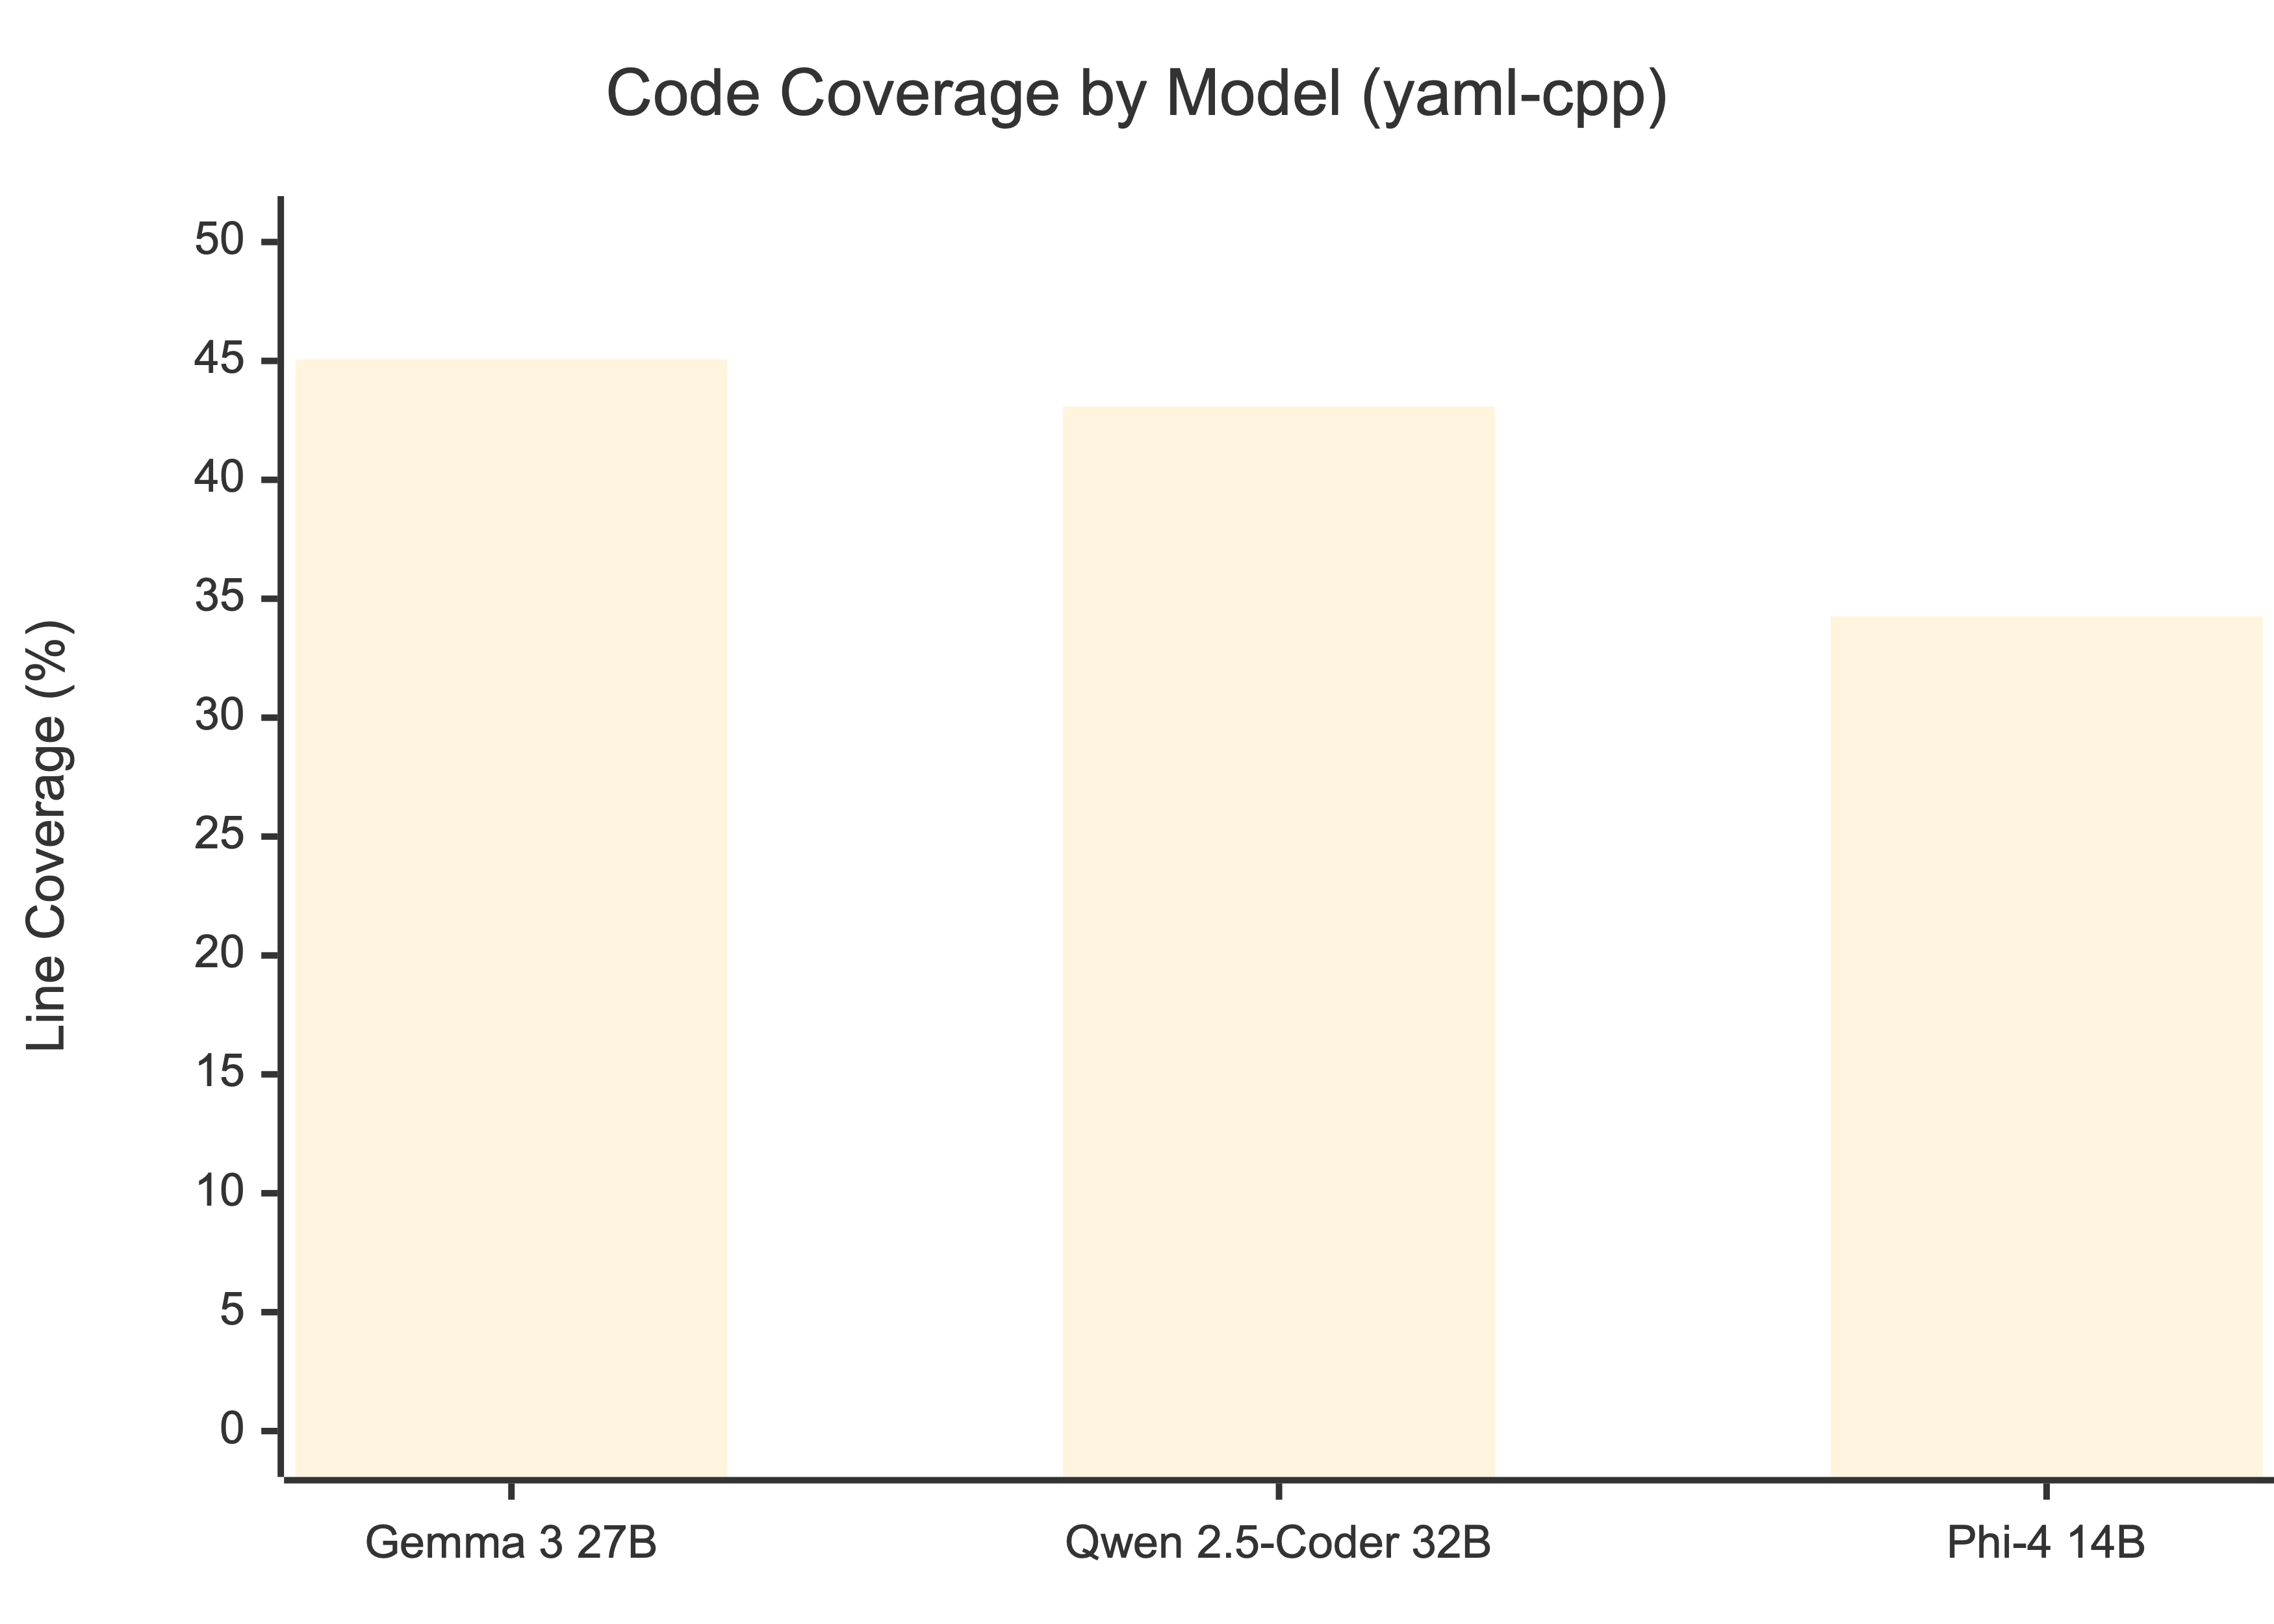
\includegraphics[width=\linewidth]{bilder/figure5_1_model_performance.png}
\end{figure}


\subsection{Unsuccessful Models: Critical Findings}
\label{sec:results_unsuccessful}

Several models did not produce usable output, as summarized in Table~\ref{tab:unsuccessful_models}. This was one of the more important findings of the research.

\begin{table}[htbp]
\centering
\caption{Unsuccessful Models and Failure Analysis on yaml-cpp}
\label{tab:unsuccessful_models}
\resizebox{\textwidth}{!}{%
\begin{tabular}{llll}
\toprule
Model & Parameters & Failure Stage & Failure Reason \\
\midrule
Qwen 2.5-Coder 14B & 14B & Compilation & Incorrect API usage, missing includes \\
Qwen 2.5-Coder 7B & 7B & Compilation & Incomplete driver structure \\
Qwen 2.5-Coder 1.5B & 1.5B & Compilation & Insufficient context understanding \\
DeepSeek Coder 33B & 33B & Compilation & Wrong function signatures \\
DeepSeek Coder V2 Lite & 16B & Compilation & Incomplete driver output \\
CodeLlama 34B Instruct & 34B & Compilation & Structural errors in generated code \\
WizardCoder 34B & 34B & Compilation & Malformed driver structure \\
Yi 34B & 34B & Runtime & Generation hallucinations, 0\% coverage \\
Gemma 3 9B & 9B & Compilation & Insufficient model capacity \\
Gemma 3 4B & 4B & Compilation & Insufficient model capacity \\
Mixtral 46.7B & 46.7B & Infrastructure & Model exceeded available hardware capacity \\
\bottomrule
\end{tabular}%
}
\end{table}

The majority of models failed at the compilation stage, producing code with syntax errors, incorrect API usage, or incomplete driver structures. Yi~34B was a notable exception: it produced code that compiled in some cases but achieved zero percent coverage at runtime. The generated drivers were syntactically valid but did not exercise the target library effectively. Functions were called with incorrect parameter combinations, or the driver simply returned immediately without exercising any library functionality. We tested variations of the prompt template to verify this was not a prompt engineering issue, and selected the version that most consistently produced compilable output. The results were consistent across attempts.

We also tested DeepSeek~R1, a reasoning-focused model, outside the original 14-model benchmark. It was designed for reasoning tasks, but in our experiments, that capability did not translate to effective fuzz driver generation. Mixtral's 46.7 billion parameters exceeded the available hardware capacity, preventing completion of a full evaluation run.

A clear pattern emerged from Table~\ref{tab:unsuccessful_models}. Code-specialized models outperformed larger general-purpose models by wide margins. Size alone does not determine quality for specialized tasks like fuzz driver generation. Furthermore, even among code-specialized models, only those with sufficient training on relevant code patterns (such as Qwen~2.5-Coder 32B) succeeded, while others (CodeLlama 34B, WizardCoder 34B) failed despite their code-focused training.


\subsection{Cross-Library Validation}
\label{sec:results_cross_library}

To validate whether the yaml-cpp findings generalize to other libraries, we tested the top-performing models on additional C++ targets. Not all models were evaluated on every library due to time constraints, so we focused on the models that showed the most promise.

\textbf{fmt (formatting library):}

Table~\ref{tab:fmt_results} presents the results for the fmt library. In addition to the 14 models from our primary benchmark, we tested Llama~3 and Qwen~1.5~7B on fmt to broaden coverage across model families.

\begin{table}[htbp]
\centering
\caption{Model Performance on fmt Library}
\label{tab:fmt_results}
\small
\begin{tabular}{lcccc}
\toprule
Model & Code Coverage & Time Taken & Tokens Used & Result \\
\midrule
Phi-4 14B & 100\% & 12m 8s & 59.8k & Successful \\
Llama~3 & 100\% & 3m 41s & 27.6k & Successful \\
Qwen~1.5 7B & 89.47\% & 6m 9s & 50k & Successful \\
Qwen 2.5-Coder 32B & 0\% & 43m 20s & 59.8k & Unsuccessful \\
Gemma 3 27B & 0\% & 41m 59s & 73.9k & Unsuccessful \\
\bottomrule
\end{tabular}
\end{table}

Table~\ref{tab:fmt_results} presents results that are counterintuitive compared to the findings from Section~\ref{sec:results_successful}. The two best-performing models on yaml-cpp (Qwen~2.5-Coder 32B and Gemma~3 27B) both achieved 0\% on fmt, while smaller models achieved near-perfect coverage.

We examined the generated outputs to understand this reversal. The fmt library exposes a small, well-documented API surface with clear input/output contracts (e.g., \texttt{fmt::format(format\_string, args...)}). The smaller models generated concise drivers that directly called these formatting functions with the fuzzer-provided input. In contrast, the larger models generated verbose, over-engineered drivers that attempted to construct complex formatting scenarios but introduced compilation errors or invalid API sequences in the process. Specifically, Qwen~2.5-Coder 32B generated drivers that referenced internal fmt implementation details not exposed in the public headers, while Gemma~3 27B produced drivers that called deprecated or non-existent overloads.

This observation is consistent with findings by Zhang et al.~\cite{LLMDriverGenEffectiveness2023}, who reported that LLM-generated fuzz drivers for simpler APIs achieve higher success rates, and that larger models do not uniformly outperform smaller ones across different target complexities. The key factor appears to be the match between model output verbosity and API complexity: simpler APIs benefit from concise, targeted generation, while complex APIs like yaml-cpp require the broader context understanding that larger models provide. This finding reinforces that no single model dominates across all library types, and model selection should consider the target API characteristics.

\textbf{pugixml (XML processing library):}

The results for fuzz-testing code from the pugixml library are presented in Table~\ref{tab:pugixml_results}.

\begin{table}[htbp]
\centering
\caption{Model Performance on pugixml Library}
\label{tab:pugixml_results}
\small
\begin{tabular}{lcccc}
\toprule
Model & Code Coverage & Time Taken & Tokens Used & Result \\
\midrule
Qwen 2.5-Coder 32B & 34.77\% & 37m 24s & 43.1k & Successful \\
Gemma 3 27B & 0\% & 1h 12m 8s & 122k & Unsuccessful \\
\bottomrule
\end{tabular}
\end{table}

On pugixml, Qwen 2.5-Coder 32B achieved 34.77\% coverage, comparable to its yaml-cpp performance (43.08\%). Gemma 3 27B did not achieve any coverage despite consuming considerably more tokens (122k vs 40.2k on yaml-cpp), suggesting the XML parsing API posed challenges that the model was not able to address in this configuration.

\textbf{jsoncons, glm, and spdlog (Qwen 2.5-Coder 32B only):}

Table~\ref{tab:additional_libraries} summarizes the results for testing jsoncons, glm, and spdlog.

\begin{table}[htbp]
\centering
\caption{Qwen 2.5-Coder 32B Performance Across Additional Libraries}
\label{tab:additional_libraries}
\resizebox{\textwidth}{!}{%
\begin{tabular}{lccccc}
\toprule
Library & Code Coverage & Time Taken & Tokens Used & Test Cases & Successful Tests \\
\midrule
jsoncons & 45.64\% & 37m 24s & 43.1k & 2,500 & 1 \\
glm & 0\% & 42m 55s & 56.8k & 0 & 0 \\
spdlog & 0\% & 49m 33s & 62.9k & 0 & 0 \\
\bottomrule
\end{tabular}%
}
\end{table}

As shown in Table~\ref{tab:additional_libraries}, jsoncons showed the highest coverage of any library we tested (45.64\%), slightly exceeding even yaml-cpp. Both are parsing libraries with similar API patterns, which may explain the consistency. glm (a mathematics library for graphics) and spdlog (a logging library) both produced 0\% coverage, indicating that the models did not generate effective drivers for non-parsing API patterns. Libraries with mathematical or configuration-heavy interfaces appear more challenging for current LLMs.

\textbf{Cross-library summary:} The results show that model performance varies considerably across libraries. Parsing libraries (yaml-cpp, jsoncons, pugixml) consistently produced the highest coverage, while utility libraries (glm, spdlog) were more challenging. Library complexity did not always predict difficulty, as fmt's simpler API yielded perfect coverage with smaller models. These findings suggest that API style and documentation quality matter more than library size or domain.


\section{Model Optimization Results}
\label{sec:results_optimization}

Having established that specialized models outperform general-purpose ones, we investigated whether fine-tuning could further improve efficiency while reducing computational requirements. These experiments address the optimization aspect of \textbf{RQ2}: can smaller models with domain-specific training match or exceed larger general-purpose models?

\subsection{LoRA Fine-Tuning Efficiency}
\label{sec:results_lora_efficiency}

Based on Phase 1 results, we selected the Qwen 2.5-Coder 1.5B model for fine-tuning experiments. The goal was to determine whether a small, fine-tuned model could match larger models while using markedly fewer resources.

We applied Low-Rank Adaptation (LoRA) \cite{Hu2021} fine-tuning using fuzz drivers from Google's OSS-Fuzz project as training data. LoRA works by freezing most of the original model weights and inserting small trainable matrices into the attention layers, so only a fraction of parameters are updated during training. This makes fine-tuning feasible on consumer hardware without the memory requirements of full model training. Our approach builds on recent work in LLM-based fuzzing \cite{llm4fuzz,TitanFuzz2022} but applies more aggressive model compression through fine-tuning. We curated two training datasets from publicly available OSS-Fuzz repositories, a small one with 172 examples and an extended one with 709 examples. Each example consisted of a fuzz driver paired with its target API context, covering security vulnerability patterns, fuzzing techniques, and automotive-specific code patterns.

Our fine-tuning configuration:
\begin{itemize}
    \item LoRA Rank: 16
    \item LoRA Alpha: 32
    \item Dropout: 0.1
    \item Target Modules: q\_proj, v\_proj, k\_proj, o\_proj
    \item Precision: float16
\end{itemize}

Results showed measurable efficiency improvements:

\begin{table}[htbp]
\centering
\caption{LoRA Fine-Tuning Efficiency Improvements}
\label{tab:lora_efficiency}
\small
\begin{tabular}{lccc}
\toprule
Model Version & Time Taken & Tokens Used & Efficiency Improvement \\
\midrule
Base 1.5B & 15 min & 112k & Baseline \\
172 examples & 12 min & 65k & 20\% faster, 42\% fewer tokens \\
709 examples & 10 min & 50k & 33\% faster, 55\% fewer tokens \\
\bottomrule
\end{tabular}
\end{table}

With 709 examples, the extended dataset produced the largest improvements with 33\% faster generation and 55\% fewer tokens compared to the base model. The fine-tuned model learned to generate more concise, targeted code rather than verbose outputs padded with unnecessary boilerplate.


\subsection{Comparative Analysis}
\label{sec:results_lora_analysis}

Training data quality and quantity both matter, though quality appears more important. The 709-example dataset outperformed the 172-example dataset, but the improvement was incremental rather than dramatic. More diverse examples help the model generalize, but there are diminishing returns.

One key insight is that a fine-tuned small model can match larger models while using markedly fewer computational resources. This makes enterprise deployment practical, as it does not require expensive GPU infrastructure to run effective fuzz driver generation.

However, we should note the limitations. The fine-tuned 1.5B model still does not match the coverage achieved by the larger Qwen 32B or Gemma 27B models. What it offers is efficiency, acceptable coverage at much lower cost and resource requirements.

The efficiency gains from fine-tuning directly impact deployment feasibility in resource-constrained environments. However, efficiency alone does not determine practical viability, cost considerations also play a major role in enterprise adoption.


\section{Economic Analysis and Resource Metrics}
\label{sec:results_economics}

Beyond technical performance, successful enterprise deployment requires favorable economics. This section addresses the cost component of \textbf{RQ3}: Can LLM-assisted fuzz driver generation be integrated into secure enterprise CI/CD pipelines while meeting performance, cost, and security requirements? As defined in Chapter~4 (Section~\ref{sec:impl_phase3}), the performance requirements include completing driver generation within the 15 to 30 minute CI/CD feedback window, the cost requirements cap annual infrastructure spending below \euro{}2,000, and the security requirements mandate that no proprietary source code leaves the corporate network. We analyzed both direct infrastructure costs and opportunity costs relative to manual approaches.

We analyzed costs in detail because the question is not only ``does this work?'' but ``is this economically viable for real deployment?''

\subsection{Azure OpenAI Cost Projections}
\label{sec:results_cost_azure}

Based on Azure OpenAI pricing as of July 2025 (the time of our experiments):

\begin{table}[htbp]
\centering
\caption{Azure OpenAI Cost Projections for Different Usage Levels}
\label{tab:cost_scenarios}
\small
\begin{tabular}{lcccc}
\toprule
Usage Level & Daily Cost & Monthly Cost & Annual Cost & Use Case \\
\midrule
Light & \euro{}0.28 & \euro{}6.16 & \euro{}73.92 & Development/testing \\
Moderate & \euro{}0.83 & \euro{}18.26 & \euro{}219.12 & Small team production \\
Heavy & \euro{}2.75 & \euro{}60.50 & \euro{}726.00 & Full enterprise deployment \\
Enterprise & \euro{}5.50 & \euro{}121.00 & \euro{}1,452.00 & Complete automation \\
\bottomrule
\end{tabular}
\end{table}

Even at the enterprise level with complete automation, annual costs stay under \euro{}1,500. This is minimal compared to manual security testing approaches. However, this represents only the direct infrastructure costs.


\subsection{Comparison with Manual Testing}
\label{sec:results_cost_manual}

Industry estimates for manual fuzz driver development:
\begin{itemize}
    \item Senior security engineer hourly rate: \euro{}80 to 120 (based on published industry benchmarks)
    \item Time to write an effective fuzz driver: 2 to 8 hours per target (lower end for well-documented parsing APIs, upper end for complex C++ libraries with heavy template usage)
    \item Annual cost for security engineering resources: varies by market and seniority
\end{itemize}

The AI-driven approach offers:
\begin{itemize}
    \item Infrastructure cost: \euro{}219-\euro{}1,452 annually
    \item Estimated time savings: 75 to 94\% reduction in initial driver creation time (based on comparison of approximately 30 minutes automated generation vs. 2 to 8 hours of manual writing per target)
\end{itemize}

The economic advantage appears clear, but there is an important caveat. Current LLMs do not incorporate domain-specific automotive safety requirements, do not account for ISO 26262 compliance considerations, and may occasionally generate tests that are syntactically correct but lack semantic depth. It should be noted that none of the test cases in our evaluation incorporated safety-related constraints (e.g., ASIL levels, timing requirements, or fault-tolerance checks); all generated drivers focused exclusively on functional correctness and coverage of the public API surface. Human oversight remains essential. The time savings estimate assumes engineers spend their time reviewing and improving AI-generated drivers rather than writing from scratch, not that AI fully replaces human judgment. The cost of this human oversight is not captured in the infrastructure costs above, and the actual savings will vary depending on the complexity of the target library and the quality of the generated driver.


\section{Summary}
\label{sec:results_summary}

The experiments produced several clear findings, along with some important caveats.

Model specialization matters more than size. Gemma 3 27B outperformed Yi 34B despite having fewer parameters. Code-specialized models outperformed larger general-purpose models consistently across our tests.

Performance also varies across library types. Parsing libraries (yaml-cpp, jsoncons, pugixml) consistently produced the best coverage results, while utility libraries (glm, spdlog) proved more challenging. The fmt library revealed that smaller models can outperform larger ones on simpler APIs, with Phi-4 14B and Llama~3 achieving 100\% coverage where the larger Qwen~2.5-Coder 32B and Gemma~3 27B both achieved 0\%.

Fine-tuning enables efficient deployment. The fine-tuned 1.5B model achieved 33\% faster generation and 55\% fewer tokens compared to the base model, though it still did not match the coverage of larger specialized models.

The economics appear favorable as well. Annual infrastructure costs range from \euro{}74 for light usage to \euro{}1,452 for full enterprise deployment. Manual security engineering involves higher personnel investment, though the two approaches serve complementary rather than interchangeable functions. The LLM automates initial driver creation while human expertise remains necessary for review and refinement.

Mapping these findings to our research questions:

\textbf{RQ1 (Effectiveness)}: Can Large Language Models generate fuzz drivers for C++ code that compile successfully, execute without errors, and achieve meaningful code coverage? The results support this at least to some extent. Our best models achieved over 40\% coverage on yaml-cpp and up to 100\% on fmt, with drivers that compiled and executed correctly. Cross-library testing (Section~\ref{sec:results_cross_library}) confirmed these results generalize to other parsing libraries like jsoncons (45.64\%) and pugixml (34.77\%), though performance on non-parsing libraries was more variable. We consider 34 to 45\% coverage ``meaningful'' because it represents automated baseline coverage that would otherwise require 2 to 8 hours of manual engineering per target. While this falls short of expert human-written drivers (60 to 80\% coverage), the value lies in automation at scale, not matching human experts.

\textbf{RQ2 (Optimization)}: Does model size determine fuzz driver quality, or can smaller models with domain-specific training match or exceed larger general-purpose models? Smaller specialized models consistently outperformed larger general-purpose models. Fine-tuning further improved efficiency, though not coverage.

\textbf{RQ3 (Feasibility)}: Can LLM-assisted fuzz driver generation be integrated into secure enterprise CI/CD pipelines while meeting performance, cost, and security requirements? Integration proved feasible at costs under \euro{}1,500 annually, but the process required careful infrastructure planning (Azure Private Link) to meet the security requirements of regulated environments.
% File: chapters/discussion.tex

\chapter{Discussion and Conclusion}
\label{chap:discussion}

This chapter interprets the experimental results from Chapter 5, connects them to the research questions posed in Chapter 1, and examines what the findings mean for practitioners. We discuss both successes and failures, then close with recommendations for future research and a summary of contributions.


\section{Interpretation of Results}
\label{sec:discussion_interpretation}

\subsection{What the Data Reveals}
\label{sec:discussion_data}

The experimental results revealed patterns we did not anticipate at the outset of this work.

Most surprising was the inverse relationship between model size and performance. Conventional wisdom in machine learning suggests larger models perform better. Our fuzz driver experiments showed something different.

Why did the larger general-purpose models fail while smaller specialized ones succeeded? We analyzed the generated code outputs and identified a consistent pattern. The larger models generated code that appeared syntactically plausible but did not align with the structural requirements of the fuzz driver task. They would create elaborate test scaffolding, call APIs in reasonable sequences, but miss the essential structure that a libFuzzer driver requires. The \texttt{LLVMFuzzerTestOneInput} function signature was wrong. The input parsing was incorrect.

Qwen 2.5-Coder succeeded because it was trained specifically on code generation tasks. It understood the structural patterns of fuzz drivers from its training data. The model had seen enough examples of the correct form to reproduce it reliably. This matters more than raw parameter count.

The LoRA fine-tuning results reinforced this insight. A small 1.5 billion parameter model, after adaptation on high-quality OSS-Fuzz drivers, produced outputs matching the quality of much larger models while using markedly fewer resources. Specialized knowledge compensated for reduced parameter count.

These findings challenge a common assumption in AI deployment. Organizations often select the largest model available, assuming a higher parameter count correlates with better results. Our data suggests this does not hold for specialized code generation tasks. A well-chosen smaller model, possibly with domain-specific fine-tuning, can match or exceed larger alternatives at a fraction of the cost.

What about the coverage numbers? The original thesis proposal considered that achieving even 40\% coverage while saving hours of expert time would constitute meaningful progress. By this standard, the automated approach succeeded. However, as discussed in Chapter 5, our examination of comparable manually-written fuzz drivers in OSS-Fuzz projects suggests expert-crafted drivers typically achieve 60 to 80\% line coverage for similar libraries, because they incorporate domain knowledge about edge cases that LLMs may miss.

This gap matters, but so does the time investment. A skilled security engineer might spend 2 to 8 hours writing and debugging a fuzz driver for a new library. Our automated pipeline generates a usable driver in approximately 30 minutes. Even if the automated driver achieves lower coverage, the time savings are meaningful.


\subsection{Unexpected Findings: Network Architecture}
\label{sec:discussion_network}

We anticipated the core technical challenge would be generating high-quality fuzz drivers. We expected difficulties with C++ complexity, API understanding, or coverage optimization. We planned our research around these expected challenges.

Infrastructure integration constituted a major focus of the implementation effort.

When we moved from local experiments to CARIAD's production environment, we identified that integrating with the corporate network architecture required additional design considerations. The CI/CD runners operated in isolated network segments by design, and external API access required explicit network path configuration. Our architecture assumed we could call LLM services from build processes, but the corporate network security policies required a tailored approach.

Resolving this required evaluating several architectural approaches. The existing proxy infrastructure was configured for approved HTTP destinations, and the runner environment was designed without VPN client capabilities, consistent with its security-hardened configuration. Caching model responses was considered but would not support dynamic code generation effectively.

We collaborated with CARIAD's infrastructure team to provision Azure Private Link endpoints. This technology creates a private connection between the corporate network and Azure services, appearing as an internal address rather than external internet. The LLM API becomes reachable without traversing the public internet.

The architecture of this solution is illustrated in Figure~\ref{fig:enterprise_network}, which shows how the Azure Private Link creates a secure tunnel between the CARIAD internal network and Azure OpenAI services, routing traffic through a private connection rather than the public internet while maintaining security compliance.

\begin{figure}[htbp]
\centering
\caption{Enterprise Network Architecture with Azure Private Link}
\label{fig:enterprise_network}
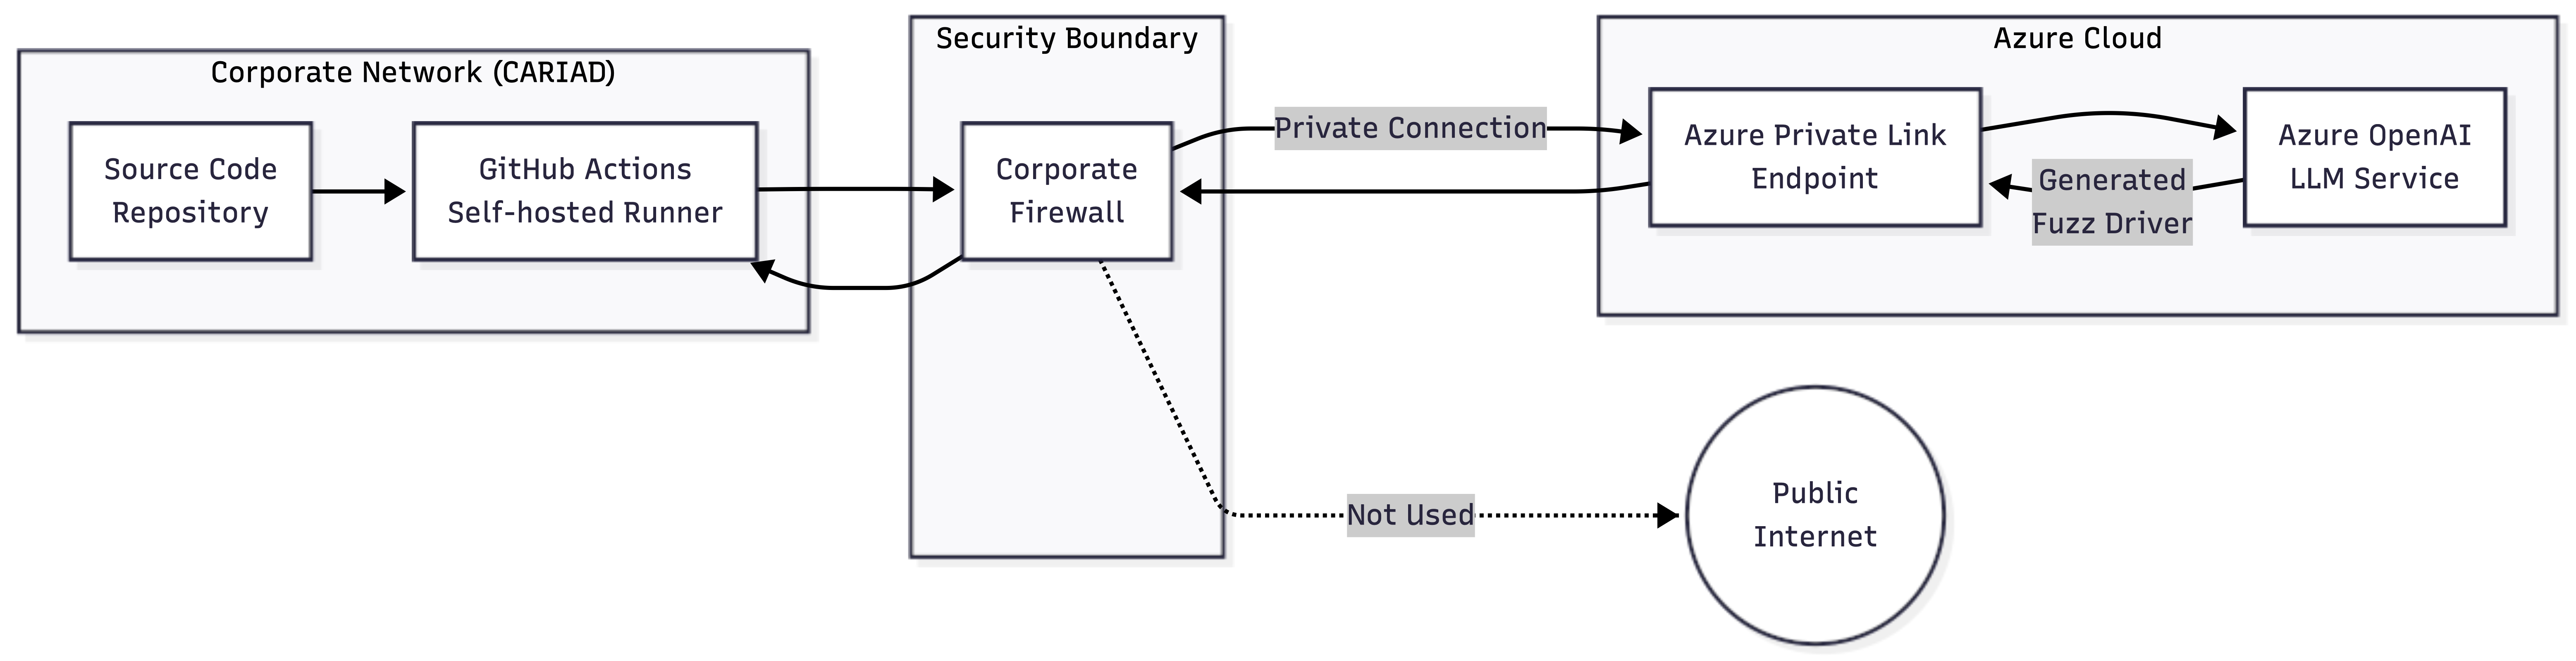
\includegraphics[width=\linewidth]{bilder/figure6_1_network_architecture.png}
\end{figure}

Setting up Private Link involved organizational coordination, including approval processes, security reviews, configuration testing, and documentation, which are standard steps for enterprise deployments in regulated industries. The technical configuration itself was manageable once approvals were obtained, requiring approximately one month from initial request to operational deployment.

This experience provided an important insight about AI deployment in enterprise environments. The machine learning components are complemented by infrastructure integration requirements. Enterprise environments introduce additional considerations, including network architecture, security compliance, and provisioning workflows, that differ from academic research settings. Anyone planning to deploy LLM-based tools in large organizations should allocate appropriate time for enterprise integration alongside the technical implementation. Based on our experience, organizations should plan for a 2- to 3-month enterprise integration timeline to accommodate standard provisioning and compliance workflows.


\section{Addressing Research Questions}
\label{sec:discussion_rq}

\subsection{Primary Research Question Analysis}
\label{sec:discussion_rq_primary}

\textbf{RQ1: Can Large Language Models generate fuzz drivers for C++ code that compile successfully, execute without errors, and achieve meaningful code coverage?}

The answer is affirmative, though several conditions apply.

The experiments demonstrated that specialized code models can generate fuzz drivers meeting these criteria. Results from Chapter 5 Section 5.2 show that the best-performing models achieved 43 to 45\% line coverage on yaml-cpp.

It is important to contextualize this finding relative to prior work. Previous studies such as TitanFuzz~\cite{TitanFuzz2022} and Fuzz4All~\cite{Fuzz4All2023} have demonstrated that LLMs can generate fuzz targets for Python libraries and deep learning frameworks. The novel contribution of our work is threefold: (1) we demonstrate this capability specifically for C/C++ libraries with libFuzzer-style drivers, which impose stricter structural requirements than Python test cases; (2) we provide a systematic comparison across 14 models showing that model selection has a decisive impact on success; and (3) we validate the approach within an enterprise CI/CD pipeline under real network isolation and security constraints, which no prior work has reported.

However, the qualifications matter. Not all models succeed. General-purpose models, even large ones, frequently did not produce usable output. Model selection matters. In practice, the question ``can LLMs do this'' should more precisely be ``which LLMs can do this, and under what conditions.''

While respectable, these coverage numbers likely trail expert human performance. LLM-generated drivers are useful for initial security testing but should not be considered equivalent to carefully crafted manual drivers for critical applications. Their advantage lies in automation speed, not coverage depth.

\textbf{RQ2: Does model size determine fuzz driver quality, or can smaller models with domain-specific training match or exceed larger general-purpose models?}

The data strongly supports the second hypothesis. Domain-specific training matters more than raw parameter count for this task.

Evidence from Chapter 5 Section 5.2 indicates that code-specialized models succeeded where larger general-purpose models did not produce usable output. Our LoRA fine-tuned 1.5B model achieved 33\% faster generation and 55\% fewer tokens while producing usable fuzz drivers (see Section 5.3). These specialized models understood what a fuzz driver should look like because they had seen relevant examples during training.

This finding has practical implications. Organizations deploying LLM-based fuzzing do not need expensive API access to the largest available models. A well-chosen mid-sized model, or a fine-tuned smaller model, provides better results at lower cost.

\textbf{RQ3: Can LLM-assisted fuzz driver generation be integrated into secure enterprise CI/CD pipelines while meeting performance, cost, and security requirements?}

Integration is feasible, but requires considerable infrastructure effort.

The performance requirement was met. As defined in Chapter~4 (Section~\ref{sec:impl_phase3}), the performance requirements specified that driver generation must complete within the 15 to 30 minute CI/CD feedback window and that fuzzing execution must not block the main build pipeline. Driver generation completed within 10 to 43 minutes depending on the model (see Table~\ref{tab:model_performance}), with the best models (Qwen~2.5-Coder 32B, Gemma~3 27B) completing in approximately 33 minutes. Fuzzing execution can run asynchronously without blocking developer feedback.

The cost requirement was met. As detailed in Chapter 5 Section 5.4, enterprise deployment costs are minimal compared to manual security testing efforts or the cost of security incidents from undetected vulnerabilities.

The security aspect required the most thorough engineering effort. Network isolation policies initially required an alternative deployment approach. The Azure Private Link solution addressed this, but required coordination with infrastructure teams. These requirements are achievable, but organizations should plan integration timelines appropriate to their specific security policies.


\subsection{Secondary Research Questions Analysis}
\label{sec:discussion_rq_secondary}

Beyond the primary questions, our work revealed answers to questions we did not explicitly ask at the start.

\textbf{What types of libraries are best suited for LLM-generated fuzz drivers?}

Experiments across multiple repositories showed that parsing libraries with clear documentation produced better drivers. Libraries with extensive header comments, consistent function signatures, and simple data types yielded higher success rates. Complex APIs with heavy template usage, deeply nested callback patterns, or implicit preconditions produced more failures.

yaml-cpp fell in the middle range. Its parsing APIs are reasonably well documented, but the YAML specification itself introduces complexity. The cross-library results from Chapter 5 Section~\ref{sec:results_cross_library} revealed additional patterns. jsoncons achieved the highest coverage (45.64\%), while the fmt library showed that smaller models can outperform larger ones when the API surface is simpler. Libraries with mathematical interfaces (glm) or configuration-heavy APIs (spdlog) consistently produced 0\% coverage, suggesting these patterns remain challenging for current LLMs.

\textbf{How do generated drivers compare to manually written ones in bug finding capability?}

We did not run extended fuzzing campaigns due to time constraints, so our evidence on this question is limited. The coverage data suggests that LLM-generated drivers explore a reasonable subset of code paths. Whether they find the same bugs as expert drivers remains an open question.

Anecdotally, during our experiments, one generated driver did trigger an assertion failure in yaml-cpp that we had not previously known about. This was a minor issue rather than a security vulnerability, but it demonstrates that automated drivers can find real problems.

\textbf{What failure modes are most common in generated drivers?}

Based on our observations during experiments, failures fell into several categories:

\begin{enumerate}
    \item Structural errors (wrong function signature, missing entry point)
    \item Type mismatches (incorrect parameter types, missing casts)
    \item Missing includes or dependencies
    \item Runtime crashes from invalid API usage
\end{enumerate}

Structural errors were the most frequent issue. The models often generated code that resembled fuzz drivers but lacked the correct \texttt{LLVMFuzzerTestOneInput} function signature or proper libFuzzer entry point structure.

The structural errors were often recoverable through prompt refinement. Adding explicit examples of correct fuzz driver structure to the prompt reduced these failures in follow-up experiments.


\section{Limitations and Constraints}
\label{sec:discussion_limitations}

\subsection{Technical Limitations}
\label{sec:discussion_tech_limits}

Our work has several technical limitations that affect how the results should be interpreted.

\textbf{Model selection scope.} We evaluated 14 open-source LLMs (plus one additional reasoning-focused model, DeepSeek R1, outside the main benchmark), but this represents a small fraction of available models. New models appear monthly, including more advanced versions of GPT-4 \cite{gpt4} and other commercial offerings we could not test due to cost or licensing considerations. Some models we did not test might perform better or worse than our selections. We chose models based on availability, documentation, and community adoption rather than exhaustive search.

\textbf{Single target language.} All experiments focused on C++ libraries. Results might differ for other languages. C has similar challenges, but Python or Rust might show different patterns due to different memory safety characteristics and training data distribution.

\textbf{Limited vulnerability discovery validation.} We measured code coverage as a proxy for fuzzing effectiveness, but coverage does not guarantee bug finding. A driver achieving 45\% coverage might miss critical code paths where vulnerabilities exist. We did not run extended fuzzing campaigns to measure actual vulnerability discovery rates.

\textbf{Hardware constraints.} Our local experiments used a single workstation with limited GPU memory. This meant we could not run the largest models at full precision. Quantization may have affected performance for some models, though we attempted to use recommended settings.

\textbf{Time constraints on fuzzing runs.} Each driver was executed for a limited time during evaluation. Longer fuzzing campaigns might reveal different coverage patterns as the fuzzer explores more deeply. Our snapshot measurements capture initial effectiveness but not long-term behavior.


\subsection{Methodological Boundaries}
\label{sec:discussion_methodology}

Beyond technical limitations, our methodology has boundaries that constrain generalization.

\textbf{Single organization context.} The enterprise integration work happened at CARIAD. Their network architecture, security policies, and tooling differ from other organizations. The specific solutions we developed (Azure Private Link, self-hosted runners) may not transfer directly to other environments.

\textbf{Limited manual driver comparison.} We compared against OSS-Fuzz drivers where available, but did not commission expert written drivers specifically for comparison. Recent research on LLM-assisted fuzzing \cite{efficient_finetuning} suggests that efficient fine-tuning can improve parameter efficiency by a large margin. The human baseline is somewhat indirect.

\textbf{No user study.} We did not evaluate how developers interact with generated drivers in practice. Do they trust the output? Do they modify it before use? These human factors affect practical deployment but were outside our scope.

\textbf{Reproducibility challenges.} LLM outputs are stochastic. Running the same prompt multiple times produces different code. We report averages across multiple generations (typically 5 runs per configuration as described in Chapter 5), but exact reproduction of our results requires matching random seeds and model versions.

These limitations do not invalidate our findings, but they define the scope within which the results apply. Organizations considering similar deployments should evaluate their specific context rather than assuming identical outcomes.


\section{Implications for Practice}
\label{sec:discussion_implications}

\subsection{Automotive Industry Impact}
\label{sec:discussion_automotive}

The automotive industry faces a particular combination of regulatory, complexity, and resource pressures that makes LLM-assisted fuzzing attractive.

Regulatory requirements are tightening. UNECE Regulation~155~\cite{UNECER155} mandates cybersecurity management systems for vehicle manufacturers. ISO/SAE~21434~\cite{ISO21434} requires systematic security engineering throughout the vehicle lifecycle. Fuzzing provides documented evidence of security testing that regulators recognize.

Software complexity continues to grow. Modern vehicles contain millions of lines of code across networked ECUs. Manual security review cannot scale to this volume.

The cost analysis from Chapter~5 Section~\ref{sec:results_economics} shows that even at the enterprise usage level, annual costs remain under \texteuro{}1,500. We recommend a phased adoption approach: start with non safety-critical subsystems like infotainment or connectivity features, build confidence and collect metrics, then gradually expand to more critical systems as the approach proves reliable.


\subsection{Enterprise CI/CD Deployment Patterns}
\label{sec:discussion_enterprise_challenges}

Our integration experience at CARIAD (detailed in Chapter~4) illustrates deployment patterns applicable to other enterprises. We identify four main approaches for integrating LLM services into security-constrained environments:

\textbf{Private deployment of models.} Running models on internal infrastructure avoids external network traffic entirely. This works for smaller models but requires dedicated compute resources. Organizations must weigh infrastructure costs against API costs.

\textbf{Cloud provider private connectivity.} Services like Azure Private Link \cite{azure_private_link}, AWS PrivateLink, and Google Cloud Private Service Connect create private paths to cloud services. These maintain security boundaries while enabling access, provided the cloud provider itself is trusted. As discussed in Chapter~4, our architecture relies on contractual trust (Microsoft Enterprise Agreement, SOC~2 Type~II, ISO~27001 certifications) rather than technical guarantees against a compromised provider. For organizations that cannot accept this trust assumption, on-premises model deployment (as evaluated in Phase~1) remains the alternative, though at higher infrastructure cost. Configuration requires coordination between cloud and enterprise network teams.

\textbf{Edge deployment.} Running models on local hardware avoids network dependencies entirely, suitable for latency-sensitive applications with infrequent model updates.

\textbf{Hybrid approaches.} Combining private deployment for sensitive operations with cloud APIs for less sensitive ones provides flexibility at the cost of additional complexity.


\section{Future Research Directions}
\label{sec:discussion_future}

Our work opens several directions for future research.

\textbf{Extended fuzzing campaigns.} We measured initial code coverage but did not run campaigns long enough to measure vulnerability discovery. Future work should execute fuzzing for hours or days, tracking crash discovery over time. This would establish whether LLM-generated drivers find bugs at rates comparable to manual drivers.

\textbf{Multi-model ensembles.} Our experiments evaluated models individually. Combining outputs from multiple models might improve quality. One model could generate initial code while another reviews and corrects it. The best combination strategy remains unexplored.

\textbf{Active learning for driver improvement.} When a generated driver fails to compile or crashes at runtime, the error messages contain useful information. Future systems could feed this information back to the LLM for iterative improvement. This closed-loop approach might achieve higher success rates than single-shot generation.

\textbf{Cross-language generalization.} We focused on C++ libraries. Extending to other languages relevant for automotive (C, Rust, Python) would broaden applicability. Different languages likely require different prompt strategies and model selections.

\textbf{Integration with other testing techniques.} LLM-generated fuzz drivers could complement symbolic execution, property-based testing, or formal verification. Understanding how to combine these approaches effectively deserves investigation.

\textbf{Human-in-the-loop workflows.} Rather than fully automated generation, interactive systems could present generated drivers to developers for review and modification. Understanding the right balance between automation and human oversight would improve practical deployment.

\textbf{Benchmark development.} The field lacks standardized benchmarks for evaluating LLM-based fuzz driver generation. Creating benchmark suites with known ground truth would enable more rigorous comparison across approaches.

\textbf{Fine-tuning data curation.} Our LoRA experiments used OSS-Fuzz drivers as training data. Systematic study of what makes good fine-tuning examples, and how much data is needed, would guide practical deployment.

\textbf{Security analysis of generated code.} LLM-generated code could contain vulnerabilities or backdoors. Analyzing the security properties of generated drivers, beyond their fuzzing effectiveness, matters for deployment in security-sensitive contexts.


\section{Contributions}
\label{sec:discussion_summary}

This thesis makes the following contributions:

\begin{enumerate}
    \item \textbf{Empirical model evaluation:} A systematic comparison of 14 LLMs for C/C++ fuzz driver generation, establishing that code-specialized models outperform larger general-purpose models (Chapter~5, Sections~\ref{sec:results_successful}--\ref{sec:results_unsuccessful}).
    \item \textbf{Fine-tuning for efficiency:} Demonstration that LoRA fine-tuning of a 1.5B model achieves 33\% faster generation and 55\% fewer tokens while maintaining driver quality (Chapter~5, Section~\ref{sec:results_optimization}).
    \item \textbf{Enterprise integration architecture:} A documented end-to-end architecture for deploying LLM-assisted fuzzing in secure enterprise CI/CD pipelines using Azure Private Link (Chapter~4, Section~\ref{sec:impl_phase3}).
    \item \textbf{Economic analysis:} A cost framework showing enterprise deployment costs remain below \texteuro{}1,500 annually (Chapter~5, Section~\ref{sec:results_economics}).
\end{enumerate}


\section{Conclusion}
\label{sec:discussion_conclusion}

This work began with a direct question, can Large Language Models automate fuzz driver generation for automotive software? After research, implementation, and deployment effort at CARIAD spanning May through September 2025, the answer is a qualified yes.

Not all models work for this task. General-purpose models, even large ones, frequently did not produce usable output. Specialized code models like Qwen 2.5-Coder succeeded where others did not. Model selection is a key design decision with measurable impact on output quality.

Fine-tuning small models proved more effective than expected. Our LoRA adapted 1.5B model achieved measurable efficiency gains (detailed in Chapter 5) while producing usable fuzz drivers. For organizations with compute constraints or cost sensitivity, this approach deserves consideration.

An important finding was the role of infrastructure. We expected the primary focus to be generating good code. In practice, a large portion of the project timeline was spent on deploying our solution within the corporate network architecture. Initial approaches including proxy configuration, boundary client integration, and container networking were iteratively refined to align with the enterprise network architecture. The solution ultimately required organizational support for Azure Private Link architecture.

Economically, adoption is well supported. As shown in Chapter 5, LLM-assisted fuzzing represents a modest investment relative to typical automotive development budgets. The value comes from scaling security testing to match code production rates that manual approaches cannot achieve.

Looking forward, LLM-assisted security testing will likely become standard practice in automotive software development. The technology works well enough today for practical deployment. It will improve as models advance and deployment patterns mature. Organizations that develop expertise now will be better positioned as the technology evolves.

For CARIAD specifically, this work establishes a foundation for expanded deployment. The architecture can accommodate additional target libraries. The cost model supports scaling. The infrastructure patterns can replicate across teams.

More broadly, our findings extend beyond fuzzing. Automotive software development faces a core scaling problem. Code complexity grows faster than team sizes. AI-assisted tools offer a path to maintain quality at scale. Fuzz driver generation is one application of this principle. Others will follow.

One key insight from this research is that infrastructure integration complexity can exceed the technical challenges of the core technology. While specific components like Azure Private Link required approximately one month for deployment, the complete enterprise integration followed standard organizational workflows for evaluation, approval, infrastructure provisioning, testing, and documentation. Organizations planning similar deployments should allocate 2 to 3 months for the full integration process and plan time commensurate with their security policy complexity.

% =========================================
% BACK MATTER
% =========================================
\appendix
\chapter{Appendix}

\section{Evaluated Model Summary}
\label{sec:appendix_models}

Table~\ref{tab:appendix_all_models} provides a complete overview of all LLM models evaluated during Phase~1 of this research, including their parameter counts, quantization levels, architecture types, and primary results on yaml-cpp.

\begin{table}[htbp]
\centering
\caption{Complete List of Evaluated Models}
\label{tab:appendix_all_models}
\resizebox{\textwidth}{!}{%
\begin{tabular}{llcccl}
\toprule
Model & Architecture & Parameters & Quantization & yaml-cpp Coverage & Status \\
\midrule
Qwen 2.5-Coder 32B & Decoder-only & 32B & Q4\_K\_M & 43.08\% & Functional \\
Gemma 3 27B & Decoder-only & 27B & Q4\_K\_M & 45.06\% & Functional \\
Phi-4 14B & Decoder-only & 14B & Q4\_K\_M & 34.26\% & Functional \\
Qwen 2.5-Coder 14B & Decoder-only & 14B & Q5\_K\_M & 0\% & Compile failure \\
Qwen 2.5-Coder 7B & Decoder-only & 7B & Q5\_K\_M & 0\% & Compile failure \\
Qwen 2.5-Coder 1.5B & Decoder-only & 1.5B & FP16 & 0\% & Compile failure \\
DeepSeek Coder 33B & Decoder-only & 33B & Q4\_K\_M & 0\% & Compile failure \\
DeepSeek Coder V2 Lite & MoE & 16B & Q4\_K\_M & 0\% & Compile failure \\
CodeLlama 34B Instruct & Decoder-only & 34B & Q4\_K\_M & 0\% & Compile failure \\
WizardCoder 34B & Decoder-only & 34B & Q4\_K\_M & 0\% & Compile failure \\
Yi 34B & Decoder-only & 34B & Q4\_K\_M & 0\% & Hallucination \\
Gemma 3 9B & Decoder-only & 9B & Q4\_K\_M & 0\% & Compile failure \\
Gemma 3 4B & Decoder-only & 4B & Q4\_K\_M & 0\% & Compile failure \\
Mixtral 46.7B & MoE & 46.7B & Q4\_K\_M & N/A & Hardware limit \\
\bottomrule
\end{tabular}%
}
\end{table}

\section{LoRA Fine-Tuning Script}
\label{sec:appendix_lora}

The following script shows the complete LoRA fine-tuning configuration used in Phase~2 (Section~\ref{sec:impl_phase2}).

\begin{lstlisting}[language=Python, caption={LoRA Fine-Tuning Script for Fuzz Driver Generation}, label={lst:appendix_lora}]
from transformers import AutoModelForCausalLM, AutoTokenizer, TrainingArguments
from peft import LoraConfig, get_peft_model
from datasets import load_dataset

# Model and tokenizer
MODEL_NAME = "Qwen/Qwen2.5-Coder-1.5B"
tokenizer = AutoTokenizer.from_pretrained(MODEL_NAME)
model = AutoModelForCausalLM.from_pretrained(MODEL_NAME, torch_dtype="float16", device_map="auto")

# LoRA configuration
lora_config = LoraConfig(
    r=16,                  # Rank: controls adaptation complexity
    lora_alpha=32,         # Scaling factor
    lora_dropout=0.1,      # Dropout to prevent overfitting
    target_modules=["q_proj", "v_proj", "k_proj", "o_proj"],
    task_type="CAUSAL_LM"
)
model = get_peft_model(model, lora_config)

# Training arguments
training_args = TrainingArguments(
    output_dir="./fuzz-lora-checkpoints",
    num_train_epochs=3,
    per_device_train_batch_size=4,
    gradient_accumulation_steps=4,
    learning_rate=2e-5,
    lr_scheduler_type="cosine",
    warmup_steps=100,
    fp16=True,
    logging_steps=10,
    save_strategy="epoch",
    evaluation_strategy="epoch",
)

# Dataset format: {"input": "<headers>", "output": "<fuzz_driver>"}
dataset = load_dataset("json", data_files="ossfuzz_drivers_709.jsonl")
\end{lstlisting}

\section{Sample Generated Fuzz Driver}
\label{sec:appendix_sample_driver}

Listing~\ref{lst:appendix_driver} shows a representative fuzz driver generated by Qwen~2.5-Coder~32B for the yaml-cpp library. This driver achieved 43\% line coverage during our evaluation (Chapter~5).

\begin{lstlisting}[language=C++, caption={Sample LLM-Generated Fuzz Driver for yaml-cpp}, label={lst:appendix_driver}]
#include <cstdint>
#include <cstddef>
#include <string>
#include "yaml-cpp/yaml.h"

extern "C" int LLVMFuzzerTestOneInput(const uint8_t *data, size_t size) {
    if (size == 0) return 0;
    
    // Convert fuzzer input to string
    std::string input(reinterpret_cast<const char*>(data), size);
    
    try {
        // Parse YAML from the fuzzer-provided input
        YAML::Node doc = YAML::Load(input);
        
        // Exercise different node types
        if (doc.IsMap()) {
            for (auto it = doc.begin(); it != doc.end(); ++it) {
                std::string key = it->first.as<std::string>();
                if (it->second.IsScalar()) {
                    std::string val = it->second.as<std::string>();
                }
            }
        } else if (doc.IsSequence()) {
            for (size_t i = 0; i < doc.size(); ++i) {
                if (doc[i].IsScalar()) {
                    std::string val = doc[i].as<std::string>();
                }
            }
        }
    } catch (const YAML::Exception&) {
        // Expected for malformed input
    } catch (const std::exception&) {
        // Catch other standard exceptions
    }
    
    return 0;
}
\end{lstlisting}

\section{Pipeline Configuration}
\label{sec:appendix_pipeline}

Listing~\ref{lst:appendix_yml} shows a simplified version of the GitHub Actions workflow used for CI/CD integration (the complete version with Azure OpenAI configuration is presented in Chapter~4, Section~\ref{sec:impl_phase3}).

\begin{lstlisting}[language=yaml, caption={GitHub Actions Workflow Snippet}, label={lst:appendix_yml}]
name: Fuzzing Pipeline
on: [push]
jobs:
  fuzz:
    runs-on: self-hosted
    steps:
      - uses: actions/checkout@v3
      
      - name: Build project
        run: |
          mkdir build && cd build
          cmake .. && make
          
      - name: Generate fuzz driver via LLM
        run: |
          cd build && cifuzz spark target_name
          
      - name: Run fuzzing
        run: |
          cd build
          cifuzz run target_name --libfuzzer-arg=-max_total_time=60
          
      - name: Collect coverage
        run: |
          cd build && cifuzz coverage target_name
\end{lstlisting}

\cleardoublepage
\phantomsection
\ifthenelse{\boolean{englishDocument}}{\renewcommand{\bibname}{References}}{\renewcommand{\bibname}{Literatur}}
\printbibliography[heading=bibintoc]

\cleardoublepage
\input{erklaerung} 

\end{document}